

\chapter{Regression and Reconstruction with Tensor-Valued
Multiway Graph Signals}

\lhead{Chapter 5. \emph{Regression and Reconstruction with
Multiway Graph Signals}}

\label{chap:nd_gsp}


Multiway Graph Signal Processing (MWGSP) is an emerging framework for analysing signals with multiple distinct axes (or `ways'), where the relation between elements within each axis is described by a graph topology \citep{Stanley2020}. For example, consider an fMRI experiment where cerebral blood flow is measured at a set of 3D voxels across time, for multiple subjects, in response to various stimuli. This dataset could be modelled as a six-way graph signal with the three spatial coordinates and the one time coordinate forming a four-way hypergrid graph, the subjects forming a graph based on characteristics, and the stimuli forming a graph based on similarity \citep{Cichocki2015}. A visual depiction of this is given in \cref{fig:fMRI_diagram}. 
 
\vspace{1.5cm}

\begin{figure}[h] 
    \begin{center}
        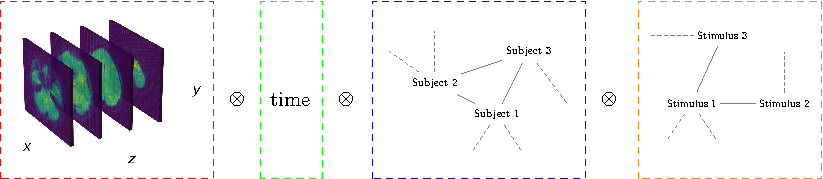
\includegraphics[width=\linewidth]{Figures/fMRI_Digaram.pdf}
    \end{center}
   \caption[Graphical depiction of an order-3 tensor]{Graphical depiction of a six-way graph signal originating from a hypothetical fMRI experiment. } 
    \label{fig:fMRI_diagram}
\end{figure} 


The goal of this chapter is to extend the methods developed in \cref{chap:gsr_2d,chap:kgr_rnc_2d} such that they can accommodate multiway graph signals. In particular, Graph Signal Reconstruction (GSR), Kernel Graph Regression (KGR) and Regression with Network Cohesion (RNC) can all be understood as a special two-dimensional case of their more general MWGSP counterpart. In this chapter, we translate all three models into their $d$-dimensional form and demonstrate how to solve efficiently for the posterior mean.  


Multiway signals are described using tensors, which can be represented as $d$-dimensional arrays. Tensor algebra is well-established in fields such as physics and mechanics \citep{Renteln2013}, however, it is less widespread in the GSP community. As such, the first section of this chapter sets out some conceptual and notational standards regarding tensors, which are core to the present and proceeding chapters. 


We begin \cref{sec:dd_gsp} by defining the Cartesian product of more than two graphs, and discuss the algebraic and spectral structure of the resultant objects. Next, we cover the tensor representation of multiway graph signals and give the general definition of graph-spectral operators in $d$-dimensions. We also discuss issues surrounding computational efficiency and how the so-called `vec-trick', utilised in prior chapters, can be generalised to the tensor setting. In \cref{sec:tensor_gsr}, we begin the core contributions of this chapter by generalising Bayesian GSR as defined in \cref{chap:gsr_2d} to the MWGSP setting. This necessitates an updated version of the SIM and CGM to accommodate tensor-valued data in arbitrary dimensions, which we give in \cref{sec:SIM_dd,sec:CGM_dd}. Next, in \cref{sec:kgr_dd}, we generalise KGR for the non-parametric prediction of multiway graph signals as a function of exogenous variables. Finally, in \cref{sec:rnc_dd}, we generalise RNC as defined in \cref{sec:rnc_mdp} in much the same way.  



\section{Multiway Graph Signal Processing}

\label{sec:dd_gsp}

\subsection{The Cartesian product of more than two graphs}

In \cref{sec:graph_products_defined} we gave the general definition of a product between two graphs and highlighted four standard examples, namely the Cartesian, direct, strong and lexicographic products. Each of these product types can be straightforwardly extended to more than two factor graphs by applying their respective definition recursively. For example, consider the Cartesian product between graphs $\mathcal{G}_A = \{\mathcal{V}_A, \mathcal{E}_A\}$, $\mathcal{G}_B = \{\mathcal{V}_B, \mathcal{E}_B\}$ and $\mathcal{G}_C = \{\mathcal{V}_C, \mathcal{E}_C\}$ where $|\mathcal{V}_A| = A$, $|\mathcal{V}_B| = B$ and $|\mathcal{V}_C| = C$. This can be written as 

\begin{equation}
    \mathcal{G} \; = \; \mathcal{G}_A \, \square \; \mathcal{G}_B \, \square \; \mathcal{G}_C \; = \; \{\mathcal{V}, \, \mathcal{E}\}
\end{equation}

The new vertex set, $\mathcal{V}$, is given by the Cartesian product of the individual vertex sets, arranged in lexicographic order. 

\begin{equation}
    \mathcal{V} = \mathcal{V}_A \times \mathcal{V}_B \times \mathcal{V}_C = \{(a, \, b, \, c) \in \mathbb{N}^3 \, | \, a \leq A, \; b \leq B, \text{and} \;  c \leq C\}
\end{equation}

The new edge set, $\mathcal{E}$, is given by recursively applying conditions 1 and 7 from, \cref{sec:graph_products_defined} to the new node set. In particular, any two nodes $(a, \, b, \, c)$ and $(a', b', c')$ are connected in $\mathcal{E}$ if they satisfy any of the following three conditions. 

\vspace{0.5cm}

\begin{table}[h]
    \def\arraystretch{1.5}
    \centering
    \begin{tabular}{lclclc}
        1. & $[a, \, a'] \in \mathcal{E}_A$    & and & $b = b'$  & and & $c = c'$             \\
        2. & $a = a'$    & and & $[b, \, b'] \in \mathcal{E}_B$   & and & $c = c'$             \\
        3. & $a = a'$    & and & $b = b'$  & and & $[c, \, c'] \in \mathcal{E}_C$              \\
    \end{tabular}
\end{table}


\begin{figure}[t]
    \begin{center}
        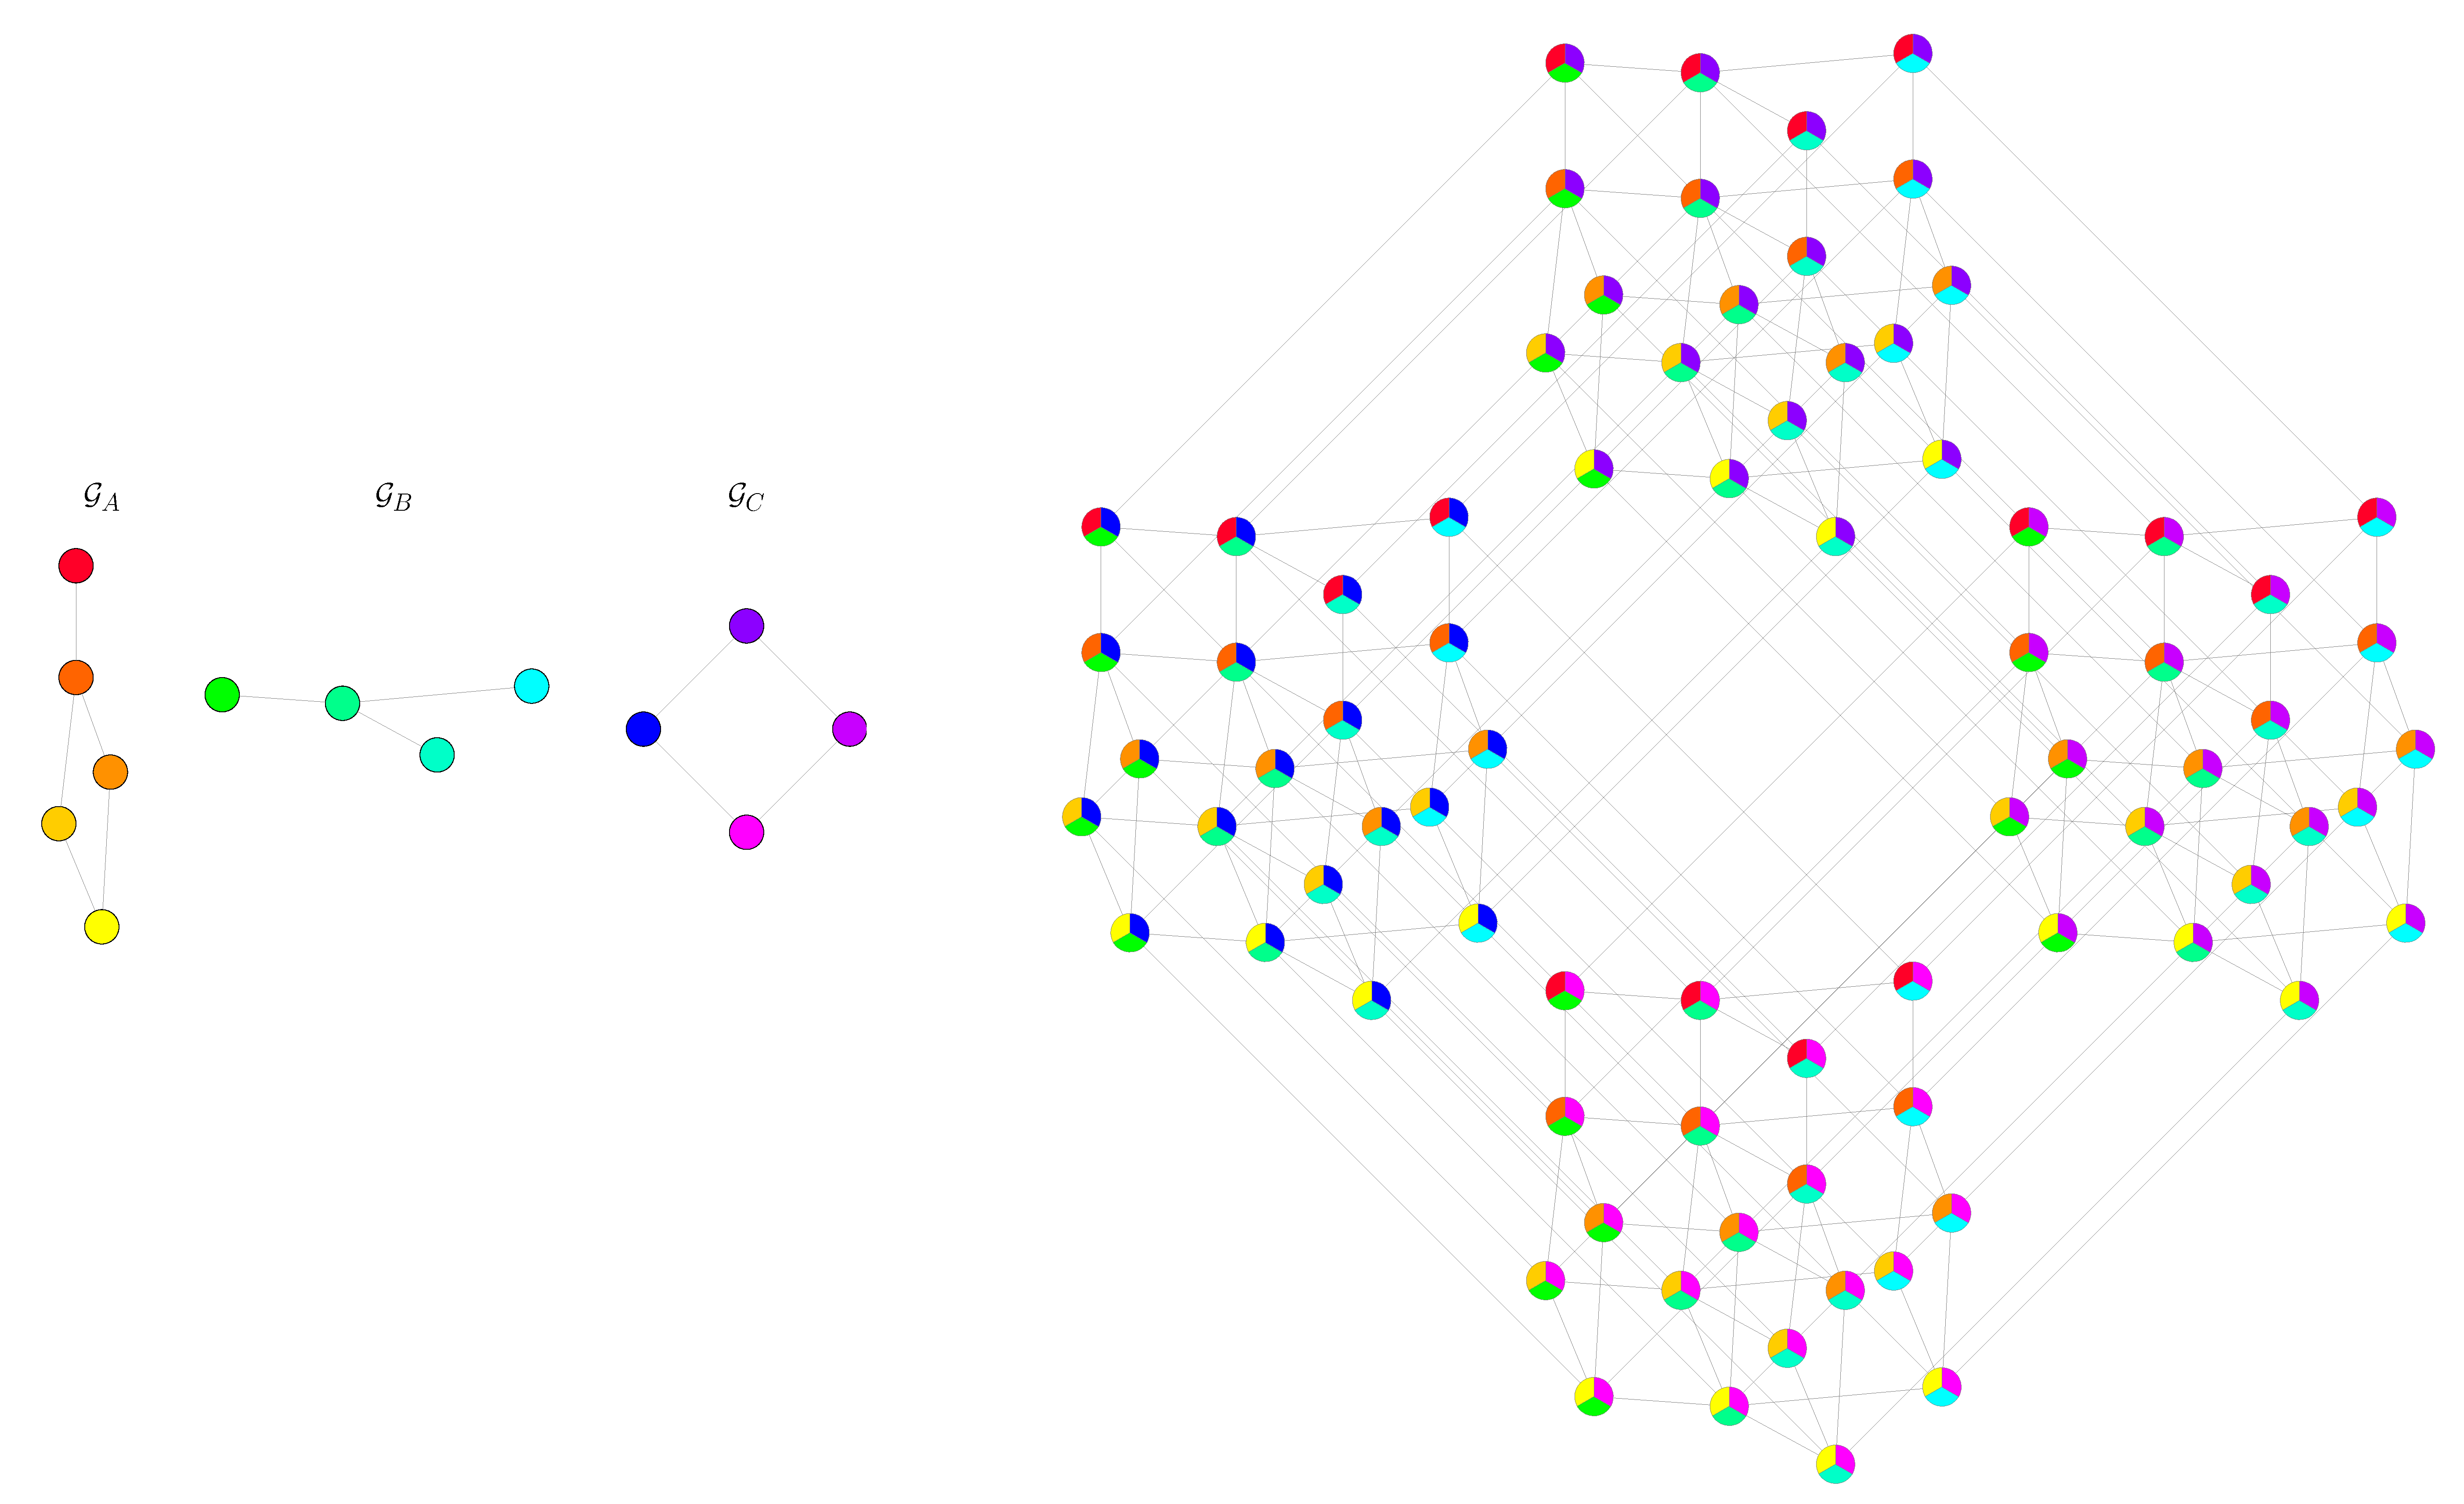
\includegraphics[width=\linewidth]{Figures/3D_CPG.pdf}
    \end{center}
    \caption[Graphical depiction of a 3D Cartesian product graph]{Graphical depiction of a 3D Cartesian product graph}
    \label{fig:3D_CPG}
\end{figure}

\Cref{fig:3D_CPG} gives a visual representation of a Cartesian product graph formed from three simple factor graphs. Notice that the size of the new vertex and edge set both grow very quickly. In particular, 

$$
|\mathcal{V}| = |\mathcal{V}_A| |\mathcal{V}_B| |\mathcal{V}_C| \aand |\mathcal{E}| =  |\mathcal{E}_A| |\mathcal{V}_B| |\mathcal{V}_C| + |\mathcal{V}_A| |\mathcal{E}_B| |\mathcal{V}_C| + |\mathcal{V}_A| |\mathcal{V}_B| |\mathcal{E}_C|
$$

Happily, the adjacency matrix of a Cartesian product graph $\A$ has a straightforward representation in terms of the factor adjacency matrices (here $\A_A$, $\A_B$ and $\A_C$). Specifically, it is given by their Kronecker sum. 

\begin{align}
    \A &= \A_A \oplus \A_B \oplus \A_C \notag \\
    &= \A_A \otimes \I_B \otimes \I_C  + \I_A \otimes \A_B \otimes \I_C + \I_A \otimes \I_B \otimes \A_C
\end{align}

In general, we can consider the Cartesian product of $d$ factor graphs with adjacency matrices denoted as $\A^{(1)} \in \R^{N_1 \times N_2}, \A^{(2)} \in \R^{N_2 \times N_2}, \dots \A^{(d)} \in \R^{N_d \times N_d}$. The full adjacency matrix will have size $N \times N$, where $N = \prod N_i$, and is given by  

\begin{alignat}{4}
    \A = \A^{(1)} & \oplus \A^{(2)} & \oplus \;\; ... \;\; & \oplus \A^{(d)} \notag \\[0.1cm]
    = \A^{(1)} & \otimes \I_{N_2} & \otimes \;\; ... \;\; & \otimes \I_{N_d} +  \notag \\[0.1cm]
    \I_{N_1} & \otimes \A^{(2)} & \otimes \;\; ... \;\; & \otimes \I_{N_d} + \;\; \ldots \;\; +  \notag \\[0.1cm]
    \I_{N_1} & \otimes \I_{N_2} & \otimes \;\; ... \;\; & \otimes \A^{(d)}  
\end{alignat}
    
This can be written compactly as 

\begin{equation}
    \A = \bigoplus_{i=1}^d  \A^{(i)}
\end{equation}

Similarly, the Laplacian of the product graph, $\LL$, can be written as the Kronecker sum of the individual factor graph Laplacians $\LL^{(i)}$. 

\begin{equation}
    \LL = \bigoplus_{i=1}^d  \LL^{(i)}
\end{equation}

We can perform eigendecomposition on each of the individual graph Laplacians as follows. 

\begin{equation}
    \LL^{(i)} = \U^{\,(i)} \LAM^{(i)} (\U^{\,(i)})^\top
\end{equation}

\noindent where $ \U^{(i)}$ is an orthogonal matrix such that each column is an eigenvector of $\LL^{(i)}$, and $\LAM^{(i)}$ is a diagonal matrix containing the corresponding eigenvalues, which are typically listed in ascending order. 

$$
\LAM^{(i)} = 
\begin{bmatrix}
    \lambda_1^{(i)}, &                 &        &                 \\
                     & \lambda_2^{(i)} &        &                 \\
                     &                 & \ddots &                 \\
                     &                 &        & \lambda_{N_i}^{(i)} \\
\end{bmatrix}
$$

Given this, the Laplacian of the product graph can be decomposed as follows. 

\begin{align}
    \LL &= \bigoplus_{i=1}^d \U^{\,(i)} \LAM^{(i)} (\U^{\,(i)})^\top \notag \\[0.2cm]
    &= \left( \bigotimes_{i=1}^d  \U^{\,(i)} \right) \left(\bigoplus_{i=1}^d \LAM^{(i)} \right) \left(\bigotimes_{i=1}^d  \U^{\,(i)} \right)^\top \notag \\[0.2cm]
    &= \U \LAM \U^\top 
\end{align}

\noindent where 

\begin{equation}
    \label{eq:U_LAM_def}
    \U =  \bigotimes_{i=1}^d  \U^{\,(i)} , \quad \text{and} \quad \LAM =  \bigoplus_{i=1}^d \LAM^{(i)}
\end{equation}


As with the Kronecker sum, here we have used the notation $\bigotimes_{i=1}^d  \U^{\,(i)}$ to denote the chained Kronecker product of matrices $\{\U^{\,(i)}  \}$. 

\subsection{Representing \textit{d}-dimensional graph signals}

Since each node in a $d$-dimensional product graph is specified by $d$ independent indices, a signal, $\Yt$, existing over the nodes has a natural representation as a tensor of order $d$. One way to conceptualise a $d$-dimensional tensor signal is as a multi-dimensional array with $d$ independent axes. If the $i$-th factor graph has $N_i$ vertices, then $\Yt$ will be of shape $(N_1, \, N_2 , ... N_d)$. An individual element of this tensor signal can be specified via a vector index $\nn = [n_1,\, n_2,\, ...,\, n_d]$, where $1\leq n_i \leq N_i$.

Alternatively, tensor signals have a dual representation as a vector of length $N = \prod N_i$. This is essential if we are to interpret the $\otimes$ symbol strictly as a Kronecker product, rather than a tensor or outer product. Under the Kronecker interpretation, the chained use of $\otimes$ used in expressions such as \cref{eq:U_LAM_def} results in matrices of shape $N \times N$, providing a linear map from $\R^{N} \rightarrow \R^{N}$. Therefore, for an operator to act on a tensor graph signal $\Yt \in \R^{N_1 \times N_2 \times ... \times N_d}$, we need a method of mapping tensors with shape $(N_1, \, N_2 , ... N_d)$ to vectors of length $N$. In order for this vectorisation process to be consistent with the operators, it should result in a vector with elements arranged in lexicographic order. In some fields, this is referred to as \textit{row-major} vectorisation since, in the case of an order-2 tensor, the index representing the row varies before the column index. In the following, we symbolise this operation mathematically as $\vecrm{\cdot}: \R^{N_1 \times N_2 \times ... \times N_d} \rightarrow \R^N$, and its reverse operation as $\tenrm{\cdot}: \R^N \rightarrow \R^{N_1 \times N_2 \times ... \times N_d}$. We use the `RM' subscript to indicate explicitly that this process is occurring in row-major order, since the standard $\vecc{\cdot}$ function defined for matrices is most commonly assumed to act in column-major order.  

In the following, we use bold lower-case symbols (e.g. $\y$) to indicate graph signals existing in their vector form, and bold upper-case calligraphic symbols (e.g. $\Yt$) to indicate graph signals in their multi-dimensional array form. That is, 

\begin{align*}
    \y = \vecrm{\Yt} \quad \Longleftrightarrow \quad \Yt  = \tenrm{\y}
\end{align*}

\Cref{fig:ten_to_vec} shows gives a visual summary of the process of converting between these two representations for an order-3 tensor. 


\begin{figure}[t]
    \begin{center}
        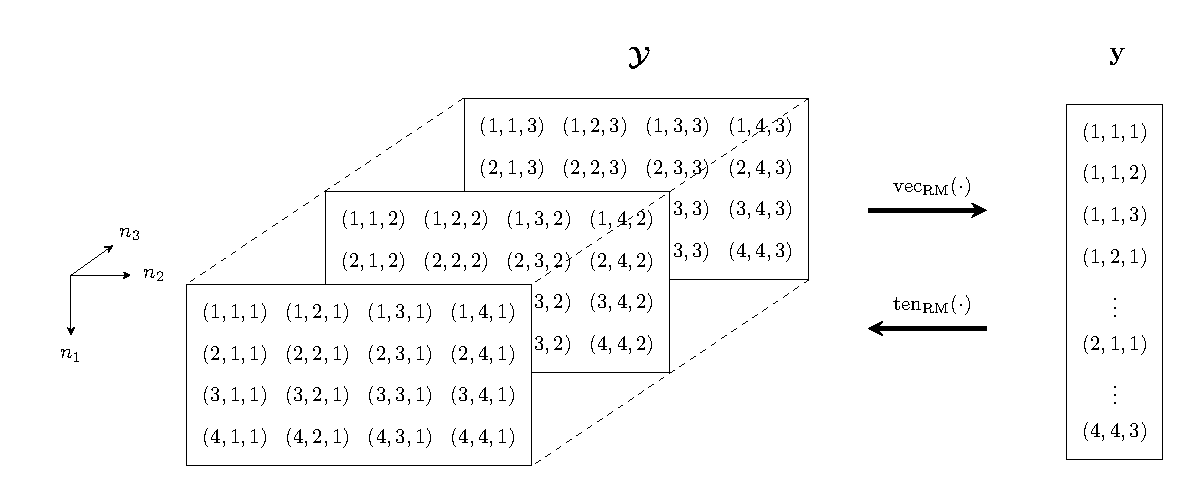
\includegraphics[width=\linewidth]{Figures/tensor_vec.pdf}    
    \end{center}
    \caption[Conversion between a multidimensional array and a vector]{A graphical depiction of the process of converting an order-3 tensor between its multidimensional array and vector form in row-major order. Note that the elements in the vectorised signal are lexicographically ordered. }
    \label{fig:ten_to_vec}
\end{figure}


To calculate the vector index $k$ which a tensor element with index $\nn = [n_1,\, n_2,\, ...,\, n_d]$ is mapped to in row-major order, we can apply the following formula.  

\begin{equation}
    \label{eq:vec}
    k = 1 + \sum_{i=1}^d \Big( \prod_{j=i+1}^d N_j \Big) \, (n_i - 1)
\end{equation}

(Note the $\pm1$ disappears when indexing begins from zero). The reverse operation, i.e. mapping a vector element index $k$ to a tensor index $\nn$ can be achieved by running the algorithm \hyperlink{vectoten}{\textbf{3}}. 


\begin{algorithm}[b]
    \hypertarget{vectoten}{}
    \label{al:vectoten}
    \caption{Mapping a vector element to a tensor element in row-major order}
    \begin{algorithmic}
    \vspace{0.15cm}
    \Require{The target vector element $k$} 
    \vspace{0.1cm}
    \Require{The shape of the output tensor $(N_1, N_2, ..., N_d)$} 
    \vspace{0.25cm}
    \State{$k \leftarrow  k - 1$}
    \vspace{0.25cm}
    \For{$i$ \textbf{from} $d$ \textbf{to} 1}
    \vspace{0.25cm}
    \State{$n_i \leftarrow  k \mod N_i$}
    \vspace{0.15cm}
    \State{$k \leftarrow \lfloor k / N_i \rfloor$} 
    \vspace{0.15cm}
    \EndFor
    \vspace{0.25cm}
    \Ensure{$(n_1 + 1, n_2 + 1, ..., n_d + 1)$}
    \end{algorithmic}
\end{algorithm}



Given these two operations, two arrays of any consistent shape can be mapped between one another by first vectorising according to \cref{eq:vec}, and then converting to a tensor using the given algorithm.

\subsection{The \textit{d}-dimensional GFT and IGFT}

\label{sec:GSP_dd}

Consider a tensor graph signal $\Yt \in \R^{N_1 \times N_2 \times ... \times N_d}$ represented in its multi-dimensional array form. In direct analogy to the two-dimensional case given in \cref{eq:GFT_2d,eq:IGFT_2d}, we can define the Graph Fourier Transform (GFT) and its corresponding inverse (IGFT) of this signal as follows. 

\begin{alignat}{2}
\label{eq:gft_nd}
    \text{GFT}(\Yt) & = \tenrm{\U^\top \y} && = \tenrm{\left(  \bigotimes_{i=1}^d  \U^{\,(i)} \right)^\top \vecrm{\Yt} } \\
\label{eq:igft_nd}
    \text{IGFT}(\Yt) & = \tenrm{\U \y} && = \tenrm{\left(  \bigotimes_{i=1}^d  \U^{\,(i)} \right) \vecrm{\Yt} }
\end{alignat}

Consider the definition of the GFT and IGFT of a $d$-dimensional graph signal given in \cref{eq:gft_nd,eq:igft_nd}. In both cases, we are required to compute the result of a chained Kronecker product matrix acting on a length-$N$ vector. Whilst the most straightforward approach to computing this product would have time and memory complexity of $O(N^2)$, a much more efficient implementation can be achieved by taking advantage of the Kronecker structure of the matrix. Specifically, the memory and time complexity of this operation can be reduced to $O(N)$ and $O(N\sum N_i)$ respectively. The importance of this fact cannot be understated, as it enables scaling to much larger product graphs than would otherwise be possible. 

This general algorithm for achieving this is well-known and can be summarised as follows. Consider the application of a chained Kronecker product matrix acting on a vector $\y$. 

$$
\y = \left( \U^{(1)} \otimes \U^{(2)} \otimes ... \otimes \U^{(d)}\right) \z
$$

This can be factorised as follows

$$
\y = \left( \U^{(1)} \otimes \I \otimes ... \otimes \I \right)\left( \I \otimes \U^{(2)} \otimes ... \otimes \I \right) ... \left( \I \otimes \I \otimes ... \otimes \U^{(d)} \right) \z
$$

As is visible, the original multiplication has now been broken into $d$ stages. However, the $i$-th stage can be completed with $N \times N_i$ multiplications by appropriately reshaping the vector and leveraging the properties of the Kronecker product. The reshaping operation can be completed using strided permutation matrices which can be applied in practice for virtually zero computational cost \citep{Granata1992}. This idea is also key to the FFT and related algorithms, which can be understood as finding a recursive Kronecker structure in the Fourier matrix \citep{Tolimieri2013}. 

Work on efficient computational procedures for this operation can be traced back to \cite{Roth1934} who formulated the original 2-dimensional ``vec trick" algorithm. The $d$-dimensional generalisation was proposed in \cite{Pereyra1973} and improved in \cite{DeBoor1979}. More recent work, such as \cite{Fackler2019}, has focused on further optimisations such as minimising data transit times and parallel processing. 

Furthermore, if the $i$-th factor graph in the Cartesian product is a path or ring graph, then the corresponding matrix transformation can be completed with only $N \log N_i$ multiplications by making use of the FCT/FST/FFT algorithms. In the extreme case, where every factor graph has this special structure, the computational complexity reaches parity with the multidimensional FFT algorithm, and will have a runtime complexity of $O(N \log N)$ \citep{Smith1995}. 

In order to execute computations of this nature in a maximally efficient way, we have developed the Python library \textit{PyKronecker}, which is described in detail in \cite{Antonian2023}. This library offers a high-level API for constructing Kronecker-based operators and applying them to either vectors or tensors, whilst optimising the underlying computation using parallel GPU processing and Just In Time (JIT) compilation using the Jax library \citep{Bradbury2018}. In the following, it will be assumed that all chained Kronecker product matrices are applied to vectors/tensors using an efficient implementation. This is essential for computing the $d$-dimensional GFT and IGFT, the basic pseudocode for which is shown in algorithm \hyperlink{al:GFT_dd}{\textbf{4}}. Note that the `reshape' operation should always be applied using the row-major convention. This is the standard convention in languages such as C and Python's NumPy library \citep{Harris2020}, but not in languages such as Matlab and Fortran which use the column major convention. 

With a fast algorithm for computing the action of a $d$-dimensional Kronecker product on a tensor defined, the corresponding algorithm for a Kronecker sum is also easily obtained. Since the Kronecker sum is defined as a sum of Kronecker products, we need only repeat this algorithm $d$ times, skipping each iteration of the loop when the corresponding product is an identity matrix. This modified form is useful when approximating filters with Chebyshev polynomials, which can be computed via repeated application of the Laplacian onto a tensor. 
 
\newpage


\begin{algorithm}[t]
    \hypertarget{al:GFT_dd}{}
    \caption{Efficient GFT and IGFT in $d$-dimensions}
    \begin{algorithmic}
    \vspace{0.25cm}
    \Require{List of Laplacian eigenvector matrices $\left\{\U^{(i)} \in \R^{N_{i} \times N_{i}}\right\}_{i=1}^d$} 
    \vspace{0.8cm}
    \Function{GFT}{$ \Yt \in \R^{N_1 \times N_2 \times ... \times N_d} $}
    \vspace{0.25cm}
    \For{$i$ \textbf{from} 1 \textbf{to} $d$}
    \vspace{0.25cm}
    \State{$\Yt\leftarrow \text{reshape}\Big(\Yt,  \;\big(N_i,\, N / N_i \big) \Big)$}
    \vspace{0.25cm}
    \State{$\Yt \leftarrow \left( \left(\U^{(i)}\right)^\top \; \Yt  \right)^\top$} 
    \vspace{0.25cm}
    \EndFor
    \vspace{0.25cm}
    \State{\textbf{return} $\text{reshape}\Big(\Yt, \; \big(N_1, \, N_2, \; ..., \; N_d \big) \Big)$}
    \vspace{0.25cm}
    \EndFunction
    \vspace{1cm}
    \Function{IGFT}{$ \Zt \in \R^{N_1 \times N_2 \times ... \times N_d} $}
    \vspace{0.25cm}
    \For{$i$ \textbf{from} 1 \textbf{to} $d$}
    \vspace{0.25cm}
    \State{$\Zt\leftarrow \text{reshape}\Big(\Zt,  \;\big(N_i,\, N / N_i \big) \Big)$}
    \vspace{0.25cm}
    \State{$\Zt \leftarrow \left( \U^{(i)} \; \Zt  \right)^\top$} 
    \vspace{0.25cm}
    \EndFor
    \vspace{0.25cm}
    \State{\textbf{return} $\text{reshape}\Big(\Zt, \; \big(N_1, \, N_2, \; ..., \; N_d \big) \Big)$}
    \vspace{0.25cm}
    \EndFunction
    \vspace{0.25cm}
    \end{algorithmic}
    \label{al:GFT_dd}
\end{algorithm}

\note{Tensor notation}{
    The use of tensor algebra is well established in fields such as physics and mechanics \citep{Renteln2013,Abraham1988}, however, it is less widespread in the signal processing community. For this reason, we choose to adopt a notation that leans more on standard linear algebra, however, all the equations and algorithms discussed in the following chapters could be alternatively written in a purer form of tensor notation. For example, consider the IGFT of a tensor signal $\Zt$. In our notation, this is written as

    \vspace{0.3cm}

    \begin{equation}
        \label{eq:LA_MM}
        \Yt = \text{ten}_{\text{RM}}\left(\left(\bigotimes_{i=1}^d  \U^{\,(i)}\right) \text{vec}_\text{RM}\left(\Zt\right) \right)    
    \end{equation}

    \vspace{0.3cm}

    As is visible, this describes the process in terms of regular matrix-vector multiplication but requires the additional definition of the $\vecrm{\cdot}$ and $\tenrm{\cdot}$ operations. Alternatively, this expression could be written using tensor indexing and Einstein summation notation as follows. 
    
    \vspace{0.3cm}

    \begin{equation}
    \label{eq:TEN_MM}
    \Yt^{\, i_1, i_2, ..., i_d} = \left(\U^{(1)}\right)^{i_1}_{j_1}\left(\U^{(2)}\right)^{i_2}_{j_2} ... \left(\U^{(d)}\right)^{i_d}_{j_d} \, \Zt^{\, j_1, j_2, ..., j_d}
    \end{equation}

    \vspace{0.3cm}

    Note that here the indices $j_1, j_2, ..., j_d$ on the right-hand side are implicitly summed over. This eliminates the need to consider vectorisation at all and is perhaps a more elegant way of describing the $d$-dimensional GFT/IGFT. However, there are multiple indices to keep track of which becomes somewhat unaesthetic in a variable number of dimensions.

    \vspace{0.3cm}
    
    Both forms offer different trade-offs, however, there is no practical difference when it comes to executing the signal processing algorithms themselves. Note that, as described in \cref{sec:GSP_dd}, the full $N \times N$ matrix implied by \cref{eq:LA_MM} is never actually instantiated in memory (see algorithm \hyperlink{KronMatMul}{\textbf{4}}).

}



\subsection{Multiway spectral operators and filtering}

\label{sec:MWGSP_filters}

In this section, we make a case for a specific restricted definition of $d$-dimensional graph filters. In \cite{Stanley2020}, the authors discuss spectral operators on multiway graph signals as functions on the space of product graph eigenvalues. We propose a specific form for such functions, which produces operators $\HH$ which can be understood as analytic functions of a Cartesian product graph Laplacian. This makes $d$-dimensional filters easier to interpret and reason about in the context of MWGSP models.  

Just as in the one and two-dimensional case, the action of a general spectral operator is computed by first taking the GFT of a signal $\Yt$, then applying some scaling function to each spectral component, and finally transforming back into the vertex domain via the IGFT. 

\begin{equation}
    \Yt' = \text{IGFT} \left( \Gt \circ \text{GFT}(\Yt) \right)
\end{equation}

The matrix operator that generates this transformation can be expressed as follows. 

\begin{equation}
    \HH = \U \, \diag{\vecrm{\Gt}} \U^\top
\end{equation}

In the most general case, the $N$ elements of $\Gt$ can vary freely to produce the total space of possible linear operators in the Laplacian eigenbasis. However, only a subset of these can be consistently interpreted as an analytic function of a Cartesian product graph Laplacian. The most restrictive possible definition of a graph filter would be one of the following form. 

\begin{align}
    \HH &= g(\beta \LL) \notag \\
        &= \U g(\beta \LAM) \U^\top
\end{align}

where 

\begin{equation*}
    \LL = \bigoplus_{i=1}^d  \LL^{(i)}, \quad \U = \bigotimes_{i=1}^d  \U^{(i)}, \aand \LAM = \bigoplus_{i=1}^d  \LAM^{(i)}
\end{equation*}

While this is a natural extension of the one-dimensional filter definition, it is isotropically constrained, since the filter strength is equal in all dimensions. In this case, the spectral scaling tensor $\Gt$ has elements $\nn = [n_1,\, n_2,\, ...,\, n_d]$ given by  

\begin{equation}
    \label{eq:Gn_dd1}
    \Gt_{\nn} = g\left(\beta\sum_{i=1}^d \lambda^{(i)}_{n_i}\right)
\end{equation}


However, we can naturally expand this to encompass anisotropic filters by introducing a parameter vector $\betaa \in \R^d$, where $\beta_i$ dictates the filter strength in the $i$-th dimension. 

\begin{align}
    \HH &= g\left( \bigoplus_{i=1}^d  \beta_i \LL^{(i)}\right)  \notag \\
        &= \U g\left( \bigoplus_{i=1}^d  \beta_i \LAM^{(i)}\right) \U^\top
\end{align}

This introduces a modified graph Laplacian $\bigoplus_{i=1}^d  \beta_i \LL^{(i)}$, which effectively scales the edge weights in each dimension by a factor of $\beta_i$. In this case, the spectral scaling tensor is given by 

\begin{equation}
    \label{eq:Gn_dd2}
    \Gt_{\nn} = g\left(\sum_{i=1}^d \beta_i \lambda^{(i)}_{n_i}\right) = g\big(\betaa^\top \lambdaa(\nn)\big)
\end{equation}

where $\lambdaa(\nn) \in \R^d$ is a vector holding the $n_i$-th eigenvalue of each graph Laplacian in the Cartesian product. 

\begin{equation}
    \label{eq:lam_of_n}
\lambdaa(\nn) = 
\begin{bmatrix}
    \lambda^{(1)}_{n_1}, & \lambda^{(2)}_{n_2}, & \dots & \lambda^{(d)}_{n_d}    
\end{bmatrix}^\top
\end{equation}

By requiring that the filter is a function of the dot product between $\betaa$ and $\lambdaa$, we effectively ensure that the operator remains consistent with the Cartesian product. Some example filters of this type are given in \cref{tab:anis_filters}. Other more general functions $g(\lambdaa)$, which do not conform to this specification, will be more difficult to strictly interpret as a filter on a Cartesian product graph Laplacian. Moreover, since filters defined in this way are analytic functions of the (axes-wise scaled) graph Laplacian, Chebyshev and other polynomial approximations can easily be leveraged to efficiently operate on signals in an eigendecomposition-free manner. However, one important caveat to note is that, while the filter strength can be varied, the functional form of the filter must be the same in each dimension. In general it is not clear how to consistently combine different functional forms for each axis into a single operator. 


\begin{table}[t]
    \def\arraystretch{1.8}
    % \small
    \begin{center}
        \begin{tabular}{lc}
            \toprule
            \textbf{Filter}   & $g(\lambdaa; \,\betaa)$ \\
            \midrule
            1-hop random walk & $(1 + \betaa^\top\lambdaa)^{-1}$\\
            Diffusion         & $\exp(-\betaa^\top\lambdaa)$\\
            ReLu              & $\max (1 - \betaa^\top\lambdaa, 0)$\\
            Sigmoid           & $2 \big( 1 + \exp(\betaa^\top\lambdaa)\big)^{-1}$\\
            Gaussian          & $\exp \big(-(\betaa^\top\lambdaa)^2\big)$\\
            Bandlimited       & $1, \,\text{if} \; \betaa^\top\lambdaa \leq 1 \; \text{else} \; 0$ \\
            \bottomrule
        \end{tabular}
    \end{center}
    \caption{Anisotropic graph filter functions in an arbitrary number of dimensions}
    \label{tab:anis_filters}
\end{table}




\section{Multiway Graph Signal reconstruction}

\label{sec:tensor_gsr}

In this section we extend the multivariate GSR model developed in \cref{chap:gsr_2d} to the MWGSP paradigm. Consider a tensor signal $\Yt$ of shape $\big(N_1, \, N_2, \, ... \, N_d \big)$ with elements interpreted as existing on the nodes of a $d$-dimensional Cartesian product graph. Only a partial set $\mathcal{S} = \{\nn_1, \, \nn_2, \, ... \}$ of the vector elements of $\Yt$ are available at observation time, with unobserved values set to zero. The goal is to estimate the signal value at these unobserved entries. 

To aid with the model description, we also introduce a binary sensing tensor $\St$, of the same shape as $\Yt$, which is used to indicate which elements of $\Yt$ were observed. This is defined as follows.  

\begin{equation}
    \St_{\nn} = \begin{cases}
        1 & \text{if} \;\; \nn \in \mathcal{S} \\
        0 & \text{otherwise}
    \end{cases}
\end{equation}

The input data for signal reconstruction on a $d$-dimensional Cartesian product graph can therefore be summarised as follows. 

\begin{equation*}
    \text{input data} = \Big\{\; \Yt \in \R^{N_1 \times ... \times N_d}, \;\; \St \in \{0, 1\}^{N_1 \times ... \times N_d} , \;\; \LL \in \R^{N \times N} \; \Big\}
\end{equation*}

In analogy with the two-dimensional case, (see \cref{sec:problem_statement_2d}), we assume that $\Yt$ is a noisy partial observation of an underlying tensor, $\Ft$, which is smooth with respect to the topology of the Cartesian product graph. This is represented by the following statistical model. 

\begin{equation}
    \Yt = \St \circ \big(\Ft + \Et \big)
\end{equation}

where, here, the $\circ$ symbol represents the generalised tensor Hadamard product, i.e. element-wise multiplication of two tensors. $\Et$ is a random tensor where each element has an independent normal distribution with unit variance. That is,

\begin{equation}
    \vecrm{\Et} \, \sim \, \Norm{\zero}{\I_N}
\end{equation}

Given this distribution over the model noise, the conditional distribution of $\Yt |  \Ft$ is given by 

\begin{equation}
    \vecrm{\Yt} \, | \, \vecrm{\Ft} \, \sim \, \mathcal{N}\Big(\vecrm{\St \circ \Ft}, \; \diag{\vecrm{\St}}\Big)
\end{equation}

Or, more concisely, 

\begin{equation}
    \y \, | \, \f \, \sim \, \mathcal{N}\big(\s \circ \f, \; \D_{\St} \big)
\end{equation}

where $\f = \vecrm{\Ft}$, $\y = \vecrm{\Yt}$ , $\s = \vecrm{\St}$ and $\D_{\St} = \diag{\s}$. In order to encode the belief that the underlying tensor $\Ft$ is smooth with respect to the topology of the graph, we can make use of the following prior distribution. 

\begin{equation}
    \f \, \sim \, \mathcal{N}\left( \zero, \, \gamma^{-1} \HH^2 \right) 
\end{equation}

where $\HH$ is constructed from an anisotropic graph filter function, with parameter $\betaa$. 

\begin{equation*}
    \HH = \U \D_\Gt \U^\top
\end{equation*}

where $\D_\Gt = \diag{\vecrm{\Gt}}$, and $\Gt$ is the spectral scaling matrix obtained by applying a graph filter to the graph Laplacian eigenvalues. The intuition for this prior can be obtained from a direct generalisation of the one and two-dimensional cases. In essence, tensor signals drawn from this prior will have the same probability density function as iid noise filtered by $\HH$, so samples will be naturally smooth with respect to the topology of the underlying Cartesian product graph. By applying Bayes' theorem, we obtain the posterior distribution for $\f$ conditioned on $\y$. 


\begin{equation}
    \f \, | \, \y \sim \Norm{\PP^{-1} \y}{\PP^{-1}}
\end{equation}

where 

\begin{equation}
    \PP = \D_{\St} + \gamma \HH^{-2}
\end{equation}

Therefore, the mean of this posterior is obtained by solving the following linear system.

\begin{equation}
    \label{eq:lin_system_dd}
    \f^{\star} = \left(\D_\St + \gamma \HH^{-2}\right)^{-1} \y
\end{equation}

Once again, we are faced with a similar set of problems to those outlined in \cref{sec:problem_statement_2d}. Namely, the coefficient matrix is very large and potentially ill-defined. This can be solved by turning to iterative methods such as the SIM and CGM, which are repeated here in their form adapted for the general tensor case. 

\subsection{Tensor SIM}

\label{sec:SIM_dd}

Generalising the SIM, which we initially describe for the two-dimensional case in \cref{sec:SIM}, to the tensor setting is straightforward. In particular, \cref{eq:lin_system_dd} can be solved by splitting the coefficient matrix $\left(\D_\St + \gamma \HH^{-2}\right)$ into $\M - \N$, where $\M$ and $\N$ take on the following values
 
\begin{equation}
    \M = \gamma \HH^{-2} + \I_N, \aand \N = \D_{\St'}
\end{equation}

where $\D_{\St'} = \diag{\mathbf{1} - \s}$. In this case, the inverse of $\M$ has the form 


\begin{align}
\M^{-1} &= \left( \bigotimes_{i=1}^d  \U^{\,(i)} \right) \, \diag{\vecrm{\Jt}}\, \left(\bigotimes_{i=1}^d  \U^{\,(i)} \right)^\top \notag \\[0.2cm]
&= \U \, \D_\Jt \, \U^\top
\end{align}

where the tensor $\Jt$ has entries with the vector index $\nn = [n_1,\, n_2,\, ...,\, n_d]$ given by 

\begin{equation}
    \Jt_{\nn} = \frac{\Gt_{\nn}^2}{\Gt_{\nn}^2 + \gamma}.
\end{equation}

Here, the entries of $\Gt$ are given by either \cref{eq:Gn_dd1} or \cref{eq:Gn_dd2}, which correspond to an isotropic or anisotropic filter function respectively. Note that, just as described in \cref{sec:SIM_cheb}, it remains possible to apply the matrix $\M^{-1}$ onto an arbitrary vector/tensor in such a way that eigendecomposition of the factor graph Laplacians is avoided entirely. This is because $\M^{-1} = J(\bigoplus \beta_i \LL^{(i)})$, where $J(x) = g^2(x) / (g^2(x) + \gamma)$, so its action can be approximated using Chebyshev polynomials. 

In a very similar manner to \cref{eq:sim_update}, the SIM update equation is given by 

\begin{equation}
    \label{eq:sim_update_dd}
    \f_{k+1} = \M^{-1}\N \f_{k} + \M^{-1} \y
\end{equation}

Note that each step can be achieved with time complexity $O(N \sum N_i)$ by making use of the fast Kronecker algorithm for computing the $d$-dimensional GFT/IFGT highlighted in \cref{sec:GSP_dd}. To be explicit, this update formula can be computed efficiently as 

\begin{align*}
    \Ft_{k+1} &= \text{IGFT} \Big( \Jt \circ \text{GFT}\big(\St' \circ \Ft_{k}\big)\Big)  + \Ft_{0} \\[0.2cm]
    \text{where} \quad \Ft_{0} &= \text{IGFT} \Big( \Jt \circ \text{GFT}\big(\Yt \big)\Big) 
\end{align*}

or, equivalently,

\begin{align*}
    \Delta \Ft_{k+1} &= \text{IGFT}  \Big( \Jt \circ \text{GFT}\big(\St' \circ \Delta \Ft_{k}\big)\Big)  \\[0.2cm]
    \text{where} \quad \Delta \Ft_{0} &= \text{IGFT} \Big( \Jt \circ \text{GFT}\big(\Yt \big)\Big)  
\end{align*}

using the fast GFT/IGFT algorithms described in \hyperlink{al:GFT_dd}{\textbf{4}}. For clarity, the full SIM algorithm is given in algorithm \hyperlink{al:SIM_dd}{\textbf{5}}. 

\begin{algorithm}[t]
    \hypertarget{al:SIM_dd}{}
    \caption{The tensor SIM for GSR}
    \begin{algorithmic}
        \vspace{0.15cm}
        \Require{Observed tensor graph signal $\Yt \in \R^{N_1 \times N_2 \times ... \times N_d}$}
        \vspace{0.15cm}
        \Require{Sensing tensor $\St \in \{0, 1\}^{N_1 \times N_2 \times ... \times N_d}$}
        \vspace{0.15cm}
        \Require{Factor graph Laplacians $\{\LL^{(i)} \in \R^{N_i \times N_i}\}_{i=1}^d $}
        \vspace{0.15cm}
        \Require{Regularisation parameter $\gamma \in \R^{+}$}
        \vspace{0.15cm}
        \Require{Graph filter function $g(\, \cdot\, \,; \betaa \in \R^{d})$}
        \vspace{0.5cm}
        \State{For $i$ from 1 to $d$, decompose $\LL^{(i)}$ into $\U^{(i)} \LAM^{(i)} \left(\U^{(i)}\right)^\top$}
        \vspace{0.15cm}
        \State{Compute $\Gt$ by applying \cref{eq:Gn_dd2}}
        \vspace{0.15cm}
        \State{Compute $\Jt$ as $\Jt_\nn = \Gt_{\nn}^2 / \big(\Gt_{\nn}^2 + \gamma\big)$}
        \vspace{0.5cm} 
        \State{$\Delta\Ft \leftarrow \text{IGFT}  \Big( \Jt \circ \text{GFT}\big( \Yt \big)\Big) $}
        \vspace{0.15cm}
        \State{$ \Ft  \leftarrow \Delta\Ft$}
        \vspace{0.15cm}
        \While{$|\Delta\Ft| > \text{tol}$}
        \vspace{0.15cm}
        \State{$\Delta\Ft \leftarrow \text{IGFT} \Big( \Jt \circ \text{GFT}\big(\St' \circ \Delta \Ft_{k} \big)\Big) $}
        \vspace{0.15cm}
        \State{$ \Ft \leftarrow  \Ft  + \Delta\Ft$}
        \vspace{0.15cm}
        \EndWhile
        \vspace{0.5cm}
        \Ensure{$ \Ft $}
        \vspace{0.15cm}
        \label{al:SIM_dd}
    \end{algorithmic}
\end{algorithm}

Once again, the worst-case scaling rate of the number of steps required for convergence, $n_{\text{SIM}}$, is bounded by

$$
\frac{1}{\log(1 + \gamma) - \log m} \; \leq \; n_{\text{SIM}} \; \leq \; \frac{1}{\log(1 + \gamma)}
$$

where $m$ is the fraction of data that is missing in the input tensor $\Yt$ (see \cref{sec:convergence}). As before, the true scaling rate will depend on the strength of the graph filter. 

\subsection{Tensor CGM}

\label{sec:CGM_dd}

The tensor version of the CGM also follows naturally from the two-dimensional case outlined in \cref{sec:CGM}. In particular, \cref{eq:lin_system_dd} can be transformed into the following equivalent preconditioned linear system. 

\begin{equation}
    \label{eq:lin_system_precon_dd}
    \f^{\star} = \PSI \left( \PSI^\top \left(\D_\St + \gamma \HH^{-2}\right)\PSI \right)^{-1}\PSI^\top \y
\end{equation}

where, in the tensor case, 

\begin{equation}
    \PSI = \left( \bigotimes_{i=1}^d  \U^{\,(i)} \right) \, \diag{\vecrm{\Gt}} = \U \D_\Gt
\end{equation}

This means \cref{eq:lin_system_precon_dd} can be expressed as 

\begin{equation}
    \f^{\star} = \PSI \left( \D_\Gt \U^\top \D_\St \U \D_\Gt + \gamma \I_N \right)^{-1}\PSI^\top \y
\end{equation}

Note that, once again, this preconditioned coefficient matrix can be multiplied onto any appropriate tensor $\Zt$ efficiently by making use of the chained Kronecker multiplication procedure given in algorithm \hyperlink{KronMatMul}{\textbf{4}}. As with the SIM, this can be performed with $O(N \sum N_i)$ multiplications. In particular, 

\begin{align*}
    \Zt' &= \tenrm{\big( \D_\Gt \U^\top \D_\St \U \D_\Gt + \gamma \I_N \big) \vecrm{\Zt}} \\[0.2cm]
    &= \Gt \circ \text{GFT} \Big( \St \circ \text{IGFT} \big(\Gt \circ \Zt\big) \Big)  + \gamma \Zt
\end{align*}


\begin{algorithm}[t]
    \hypertarget{al:CGM_dd}{}
    \caption{The tensor CGM for GSR}
    \begin{algorithmic}
        \vspace{0.15cm}
        \Require{Observed tensor graph signal $\Yt \in \R^{N_1 \times N_2 \times ... \times N_d}$}
        \vspace{0.15cm}
        \Require{Sensing tensor $\St \in \{0, 1\}^{N_1 \times N_2 \times ... \times N_d}$}
        \vspace{0.15cm}
        \Require{Factor graph Laplacians $\{\LL^{(i)} \in \R^{N_i \times N_i}\}_{i=1}^d $}
        \vspace{0.15cm}
        \Require{Regularisation parameter $\gamma \in \R^{+}$}
        \vspace{0.15cm}
        \Require{Graph filter function $g(\, \cdot\, \,; \betaa \in \R^{d})$}
        \vspace{0.5cm}
        \State{For $i$ from 1 to $d$, decompose $\LL^{(i)}$ into $\U^{(i)} \LAM^{(i)} \left(\U^{(i)}\right)^\top$}
        \vspace{0.15cm}
        \State{Compute $\Gt$ by applying \cref{eq:Gn_dd2}}
        \vspace{0.5cm} 
        \State{Initialise $\Zt$}
        \vspace{0.15cm}
        \State{$\Rt \leftarrow \Gt \circ \text{GFT} \left( \Yt \right)$}
        \vspace{0.15cm}
        \State{$\Dt \leftarrow \Rt$}
        \vspace{0.5cm}
        \While{$|\Delta\RR| > \text{tol}$}
        \vspace{0.25cm}
        \State{$\At \leftarrow \Gt \circ \text{GFT} \Big( \St \circ \text{IGFT} \big(\Gt \circ \Dt \big) \Big)  + \gamma \Dt  $}
        \vspace{0.15cm}
        \State{$\alpha \leftarrow  \sum_{\nn} \Rt_{\nn}^2 \, / \, \sum_{\nn} \Rt_\nn \At_\nn $}
        \vspace{0.15cm}
        \State{$\Zt \leftarrow  \Zt + \alpha \Dt $}
        \vspace{0.15cm}
        \State{$\Rt \leftarrow  \Rt - \alpha \At $}
        \vspace{0.15cm}
        \State{$\delta \leftarrow \sum_{\nn} \Rt_{\nn}^2  \, / \, \sum_{\nn} (\Rt + \alpha \At)^2$}
        \vspace{0.15cm}
        \State{$\Dt \leftarrow  \Rt + \delta \Dt $}
        \vspace{0.25cm}
        \EndWhile
        \vspace{0.5cm}
        \Ensure{$\text{IGFT} \left(  \Gt \circ \Zt \right)$}
        \vspace{0.15cm}
    \end{algorithmic}
    \label{al:CGM_dd}
\end{algorithm}



Just as with the two-dimensional case, we can bound the condition number of the preconditioned coefficient matrix to find the worst-case scaling rates in the limit of a weak and strong filter. As before, this falls between

$$
\sqrt{\frac{1 - m + \gamma}{\gamma}} \; \leq \; n_{\text{CGM}} \; \leq \; \sqrt{\frac{1+\gamma}{\gamma}}
$$

\section{Multiway Kernel Graph Regression}

\label{sec:kgr_dd}

In this section, we take the Kernel Graph Regression (KGR) algorithm, developed in \cref{sec:kgr_mdp}, and generalise it to the multiway/tensor case. Consider a series of $T$ product graph signals, each denoted as $\Yt_t$, with dimensions $(N_1 \times ... \times N_d)$. In this scenario, each signal is associated with an explanatory vector, $\x_t \in \R^M$. Therefore, the available data consist of labelled pairs $\big\{\x_t, \Yt_t\big\}_{t=1}^T$. This data can be consolidated into a a matrix, $\X$, of dimensions $(T \times M)$, and a tensor, $\Yt$, with shape $(T \times N_1 \times ... \times N_d)$.

The observed tensor $\Yt$ may also contain an arbitrary amount of missing data, which is described by the binary sensing tensor $\St$. In accordance with previous sections, $\St$ shares its shape with $\Yt$ and holds ones at elements where successful observations were made and zeros elsewhere. As a result, the input data for multiway KGR can be summarised as follows.

\begin{equation*}
    \text{input data} = \Big\{ \; \X \in \R^{T \times M}, \;\; \Yt \in \R^{T \times N_1 \times ... \times N_d}, \;\; \St \in \{0, 1\}^{T \times N_1 \times ... \times N_d} , \;\; \LL \in \R^{N \times N} \; \Big\}
\end{equation*}

The goal of KGR is to estimate all the missing values within $\Yt$, accounting for both the topology of the graph and the explanatory variables. As with the two-dimensional KGR model elaborated in \cref{sec:kgr_mdp}, no distinction is necessary between ``training" and ``testing" data in this context. To make a completely new prediction for some explanatory vector $\x_t$, we merely assign zero to the corresponding values in $\Yt$ and $\St$.

The fundamental logic underpinning the tensor-valued version of KGR remains consistent with the two-dimensional scenario. We continue to assume that $\Yt$ is a noisy, partial observation of an underlying latent signal $\Ft$, which is captured in the following statistical model.

\begin{equation}
    \label{eq:likelihood_kgr_nd}
    \y \, | \, \f \sim \Norm{\s \circ \f}{\I_{NT}}
\end{equation}

In this section, we omit a detailed derivation of the prior distribution over $\f$ from first principles, as the process closely resembles the steps provided in \cref{sec:kgr_mdp}. For the purposes of this section, we justify it by stating that the signal $\Ft$ should display smooth variations across both the space of explanatory variables and the topology of the Cartesian product graph. This can be encoded in the following prior distribution for $\f$.

\begin{equation}
    \label{eq:prior_kgr_nd}
    \f \sim \Norm{\zero}{\gamma \K \otimes \HH^2}
\end{equation}

In this expression, $\K$ denotes a $(T \times T)$ kernel matrix, which is created by applying a valid Mercer kernel, $\kappa$, to pairs of explanatory variables such that $\K_{ij} = \kappa(\x_i, \x_j)$. Multiple options for $\kappa$ are available, including popular choices such as the Gaussian kernel (see \cref{eq:gaussian_kernel}). By applying Bayes' rule to \cref{eq:likelihood_kgr_nd,eq:prior_kgr_nd}, the posterior distribution over the latent signal $\f$ can be established. This is given by 

\begin{equation}
    \label{eq:posterior_kgr_nd}
    \f \, | \, \y \sim \Norm{\bar{\PP}^{-1} \y}{\bar{\PP}^{-1}}
\end{equation}

where, in this case, the posterior precision matrix $\bar{\PP}$ is an $NT \times NT$ matrix given by


\begin{equation}
    \bar{\PP} = \D_\St + \gamma \K^{-1} \otimes \HH^{-2}
\end{equation}

\subsection{Computation of the posterior mean}

In order to find the posterior mean, we must solve the linear system $\bar{\PP}^{-1} \y$. Again, this can be achieved by utilising the tensor versions of the SIM or CGM. In close analogy with the two-dimensional case, the process is the same as that of multiway GSR, under the following change of variables. 

\begin{equation}
    \U \rightarrow \bar{\U}, \aand \Gt \rightarrow \bar{\Gt}
\end{equation}

To define $\bar{\U}$ and $\bar{\Gt}$, first we must define the eigendecomposition of the kernel matrix $\K$. 

\begin{equation}
    \K = \V \LAM_K \V^\top
\end{equation}

where $\V$ is the matrix with columns representing the normalised eigenvectors of $\K$, and $\LAM_K$ is the diagonal matrix holding its eigenvalues in ascending order, such that  

\begin{equation}
\LAM_K = \diag{\left[\lambda^{(K)}_1, \; \lambda^{(K)}_2, \; \dots, \;\lambda^{(K)}_T \right]}
\end{equation}

Then, $\bar{\U}$ and $\bar{\Gt}$ are defined as follows.

\begin{equation}
    \bar{\U} \in \R^{NT \times NT} = \V \otimes \U
\end{equation}

and 

\begin{equation}
    \bar{\Gt}_{t, \nn} = g(\lambdaa(\nn), \betaa) \sqrt{\lambda_t^{(K)}} \quad \Longleftrightarrow \quad \D_{\bar{\Gt}} = \LAM_K^{1/2} \otimes \D_\Gt 
\end{equation}

Just as with the to dimensional case in the previous chapter, elements of $\bar{\Gt}$ which are larger are associated with smoother eigenvectors. However now these eigenvectors span the entire product space including the product graph and the space of explanatory variables. 

From here, either the SIM or CGM, as given in \cref{al:SIM_dd,al:CGM_dd}, can be applied. The only changes necessary are the swap in $\bar{\U}$ for $\U$ and $\bar{\Gt}$ for $\Gt$. As such, this means that whenever $\text{GFT}(\cdot)$ is used, it instead signifies the following operation.  

\begin{alignat}{2}
    \label{eq:gftp_nd}
        \text{GFT}(\Yt) & = \tenrm{\bar{\U}^\top \y} && = \tenrm{\V^\top \otimes \left(  \bigotimes_{i=1}^d  \U^{\,(i)} \right)^\top \vecrm{\Yt} } \\
    \label{eq:igftp_nd}
        \text{IGFT}(\Yt) & = \tenrm{\bar{\U} \y} && = \tenrm{\V \otimes \left(  \bigotimes_{i=1}^d  \U^{\,(i)} \right) \vecrm{\Yt} }
\end{alignat}

Note that these no longer technically represent the GFT and IGFT, but a modified Kronecker operation that now includes an additional dimension described by $\V$. 

\newpage

\section{Multiway Regression with Network Cohesion}

\label{sec:rnc_dd}

In this section, we extend the Regression with Network Cohesion (RNC) and Kernel Graph Regression with Network Cohesion (KGRNC) algorithms, initially discussed in \cref{sec:rnc_mdp}, to the multiway GSP framework. Our starting point will be multiway RNC. In this context, we are concerned with a graph signal residing on the nodes of a known $d$-dimensional Cartesian product graph, where an arbitrary subset of the elements could be corrupted or absent. Furthermore, each of the $N = N_1 \times ... \times N_d$ nodes is accompanied by a length-$M$ vector of explanatory variables. Consequently, the available data can be summarised as follows.

\begin{equation*}
    \text{input data} = \Big\{ \;\Xt \in \R^{N_1 \times ... \times N_d \times M}, \;\; \Yt \in \R^{N_1 \times ... \times N_d}, \;\; \St \in \{0, 1\}^{N_1 \times ... \times N_d}, \;\; \LL \in \R^{N \times N} \; \Big\}
\end{equation*}

As before, the binary sensing tensor $\St$ describes which elements of $\Yt$ were available at observation time. We also define the matrix $\X$ which is a reshaping of the tensor of explanatory variables $\Xt$ such that

\begin{equation}
    \label{eq:X_RNC_dd}
    \X \in \R^{N \times M} = \begin{bmatrix} \vecc{\Xt_{:, 1}} & \vecc{\Xt_{:, 2}} & \dots & \vecc{\Xt_{:, M}} \end{bmatrix}    
\end{equation}

In this model, we assume that the signal $\Yt$ is a noisy partial observation of the sum of a smooth tensor signal $\Ct$ and a linear combination of the explanatory variables at each node. This is summarised in the following model. 

\begin{equation}
    \label{eq:rnc_stat_model_wc_dd}
    \y = \s \circ \big( \cc + \X \w  + \e \big)
\end{equation}

Here, $\cc \in \R^N = \vecrm{\Ct}$ is the flexible intercept term, which is assumed to vary smoothly across the $d$-dimensional product graph. $\w \in \R^{M}$ is the learned coefficient vector which specifies the contribution of the explanatory variables to the prediction at each node. $\e \in \R^N$ is a random vector of iid Gaussian noise representing the model error. As in the two dimensional case, we can stack $\cc$ and $\w$ into a single parameter vector $\thetaa$ as 

\begin{equation}
    \thetaa \in \R^{N + M} = \begin{bmatrix}
        \cc \\ \w
    \end{bmatrix}
\end{equation}

Then, the probability distribution over $\y$ given $\thetaa$ can be expressed as follows. 

\begin{equation}
    \y \, | \, \thetaa \sim \Norm{\s \circ \left(\begin{bmatrix}\I_N & \X \end{bmatrix} \thetaa \right)}{\D_\St}
\end{equation}

To create a prior over $\thetaa$, we can combine the assumption that $\Ct$ should vary smoothly over the graph with an L2 prior over the coefficient vector $\w$. This is expressed as 

\begin{equation}
    \thetaa \sim \Norm{\zero}{\begin{bmatrix}\gamma^{-1} \HH^2 & \zero \\
    \zero & \lambda^{-1} \I_M \end{bmatrix}}
\end{equation}

The resultant posterior distribution over $\thetaa$ is therefore given by 

\begin{equation}
    \thetaa \, | \, \Yt \sim \Norm{\widetilde{\PP}^{-1} \begin{bmatrix} \y \\ \X^\top \y \end{bmatrix}}{\widetilde{\PP}^{-1}}
\end{equation}

where 

\begin{equation}
    \widetilde{\PP} \in \R^{(N + M) \times (N + M)} = 
    \begin{bmatrix}
     \D_\St + \gamma \HH^{-2} & \D_\St  \X \\
     \X^\top \D_\St & \X^\top \D_\St \X + \lambda \I_M   
    \end{bmatrix}
\end{equation}

As in \cref{sec:rnc_mdp}, we can solve the linear system $\widetilde{\PP}^{-1}\begin{bmatrix} \y \\ \X^\top \y \end{bmatrix}$ using the CGM. In particular, we first define the symmetric preconditioner $\widetilde{\PSI}$ as follows. 

\begin{equation}
    \widetilde{\PSI} \in \R^{(N + M) \times (N + M)} = \begin{bmatrix}
        \U \D_\Gt & \zero \\
        \zero & \U_M \D_M 
    \end{bmatrix}
\end{equation}

where $\U_M$ and $\D_M$ are generated form the eigendecomposition of $\X^\top \D_\St \X$ as follows. 

\begin{equation}
    \X^\top \D_\St \X = \U_M \LAM_M \U_M^\top, \aand \D_M = \left(\LAM_M + \lambda \I_M\right)^{-1/2}
\end{equation}

This allows us to generate a preconditioned coefficient matrix and solve the modified linear system as follows.  

\begin{equation*}
    \widetilde{\PSI}^\top \widetilde{\PP}  \widetilde{\PSI} = 
       \begin{bmatrix}
        \D_\Gt \U^\top \D_\St \U \D_\Gt + \gamma \I_{NT}  &  \D_\Gt \U^\top \D_\St \X \U_M \D_M \\[0.1cm] 
        \D_M \U_M^\top \X^\top \D_\St \U \D_\Gt & \I_M
        \end{bmatrix}
\end{equation*}

\begin{equation*}
    \thetaa^\star = \widetilde{\PP}^{-1}\begin{bmatrix} \y \\ \X^\top \y \end{bmatrix}\, \quad \Longrightarrow \quad  \thetaa^\star = \widetilde{\PSI} \left(\widetilde{\PSI}^\top \widetilde{\PP}  \widetilde{\PSI} \right)^{-1}\widetilde{\PSI}^\top \begin{bmatrix} \y \\ \X^\top \y \end{bmatrix}
\end{equation*}


 
\newpage 

\section{GSR and KGR for green bond yield prediction}

\label{sec:green_bonds}

In this section, we undertake an analysis of the multiway Graph Signal Reconstruction and Kernel Graph Regression algorithms, developed in \cref{sec:tensor_gsr,sec:kgr_dd}, applying them to the problem of predicting the yield of a set of green bonds over time. Green finance has recently emerged as an important asset class for funding the transition to a lower carbon economy \citep{Peters2022}. Green bonds provide a mechanism for governments and municipalities to raise capital for large projects with specific climate or environmental sustainability objectives. In this case study, we utilise the yield time series for a number of US municipal green bonds, collected from Bloomberg, and attempt to estimate the missing values. This approach presents a novel method for estimating the theoretical price of bonds with various characteristics and for analysing the relationship between external factors, such as the federal funding rate or inflation, and yield. 

The yield (to maturity) of a bond is the single discount rate that, when applied to all cash flows, results in a present value equal to the current market price \citep{Hull2009}. Broadly speaking, yields represent return on investment and therefore reflect the perceived risk of a particular security, with higher yields necessary to justify riskier assets. External macroeconomic factors such as inflation, central bank interest rates, and economic uncertainty also play a key role in determining yields. 

\begin{figure}[b] 
    \begin{center}
        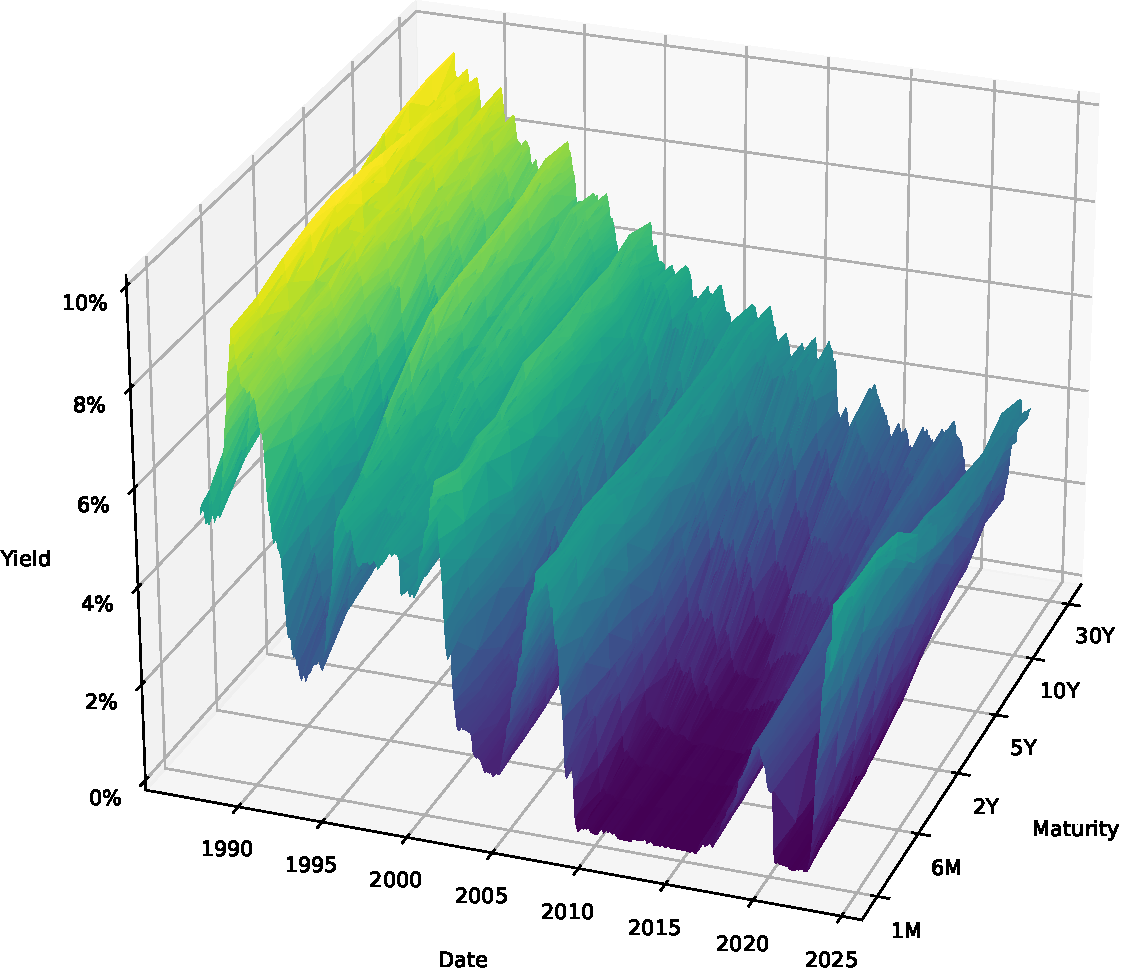
\includegraphics[width=0.75\linewidth]{Figures/fed_rates.pdf}
    \end{center}
   \caption[3D plot of the yield on US treasuries of various maturities over time]{A 3D plot of the yield on US treasuries of various maturities over time. } 
    \label{fig:US_yield_curve} 
\end{figure} 

One key intrinsic factor that can influence the yield of a bond is its maturity, representing the length of time before the principal must be repaid. Under normal market conditions, long-term fixed-income securities, such as 20-year bonds, typically provide higher returns than their short-term counterparts, such as 2-year bonds. This is primarily due to the greater uncertainty associated with longer-term securities, especially concerning potential fluctuations in future interest rates. For a set of equivalent bonds differing only based on their maturity length, the yield is expected to interpolate smoothly at any given time, forming the so-called yield curve. \Cref{fig:US_yield_curve} demonstrates how the yield curve for US treasuries has varied over the past 35 years.

For bonds issued by other entities, such as state authorities, numerous intrinsic factors other than maturity may affect the yield. These include the credit rating of the issuer, the tax exemption status, and, particularly relevant to green bonds, the Environmental, Social and Governance (ESG) impact of the funded project. In this case study, we frame the problem of estimating unknown yields as a multiway graph signal processing task. Specifically, we categorise the bonds based on several factors likely to influence the yield, such that each bond can be associated with a node on a four-dimensional Cartesian product graph. In particular, we take into account the following factors, each of which forms the basis of one of the factor graphs. 

\begin{enumerate}
    \item \textit{Use of funds}. Each bond in our dataset was associated with a project category (such as water, pollution or power) and sub-category (such as waste management, habitat conservation, or solar farms). We used this information to construct a tree graph, beginning with a root node, and branching into category and sub-category nodes. The resulting tree, comprising a total of 161 nodes, is visualised in \cref{fig:green_bond_graph}. Each bond can then be associated with a specific leaf node based on its particular project category.
    \item \textit{Credit rating}. Each bond also had an assigned credit rating associated with the issuer, designated by a ratings agency. These ratings range from the highest possible, ``AAA", to the lowest in our dataset, ``BBB+", giving a total of eight categories. Since these ratings have a natural order, they can be represented using a simple chain graph.
    \item \textit{Maturity}. Each bond has a fixed period from its issue date to the date of maturity. Unlike treasury bonds, the green bonds we considered did not necessarily have standard maturity lengths. We thus categorised each bond by the length of this period, sorted into eight different bins, with edges corresponding to 0, 1, 2, 5, 10, 20, 30, 40 and 50 years. As with credit rating, the natural order enables us to represent this with a chain graph.
    \item \textit{Tax status}. Each bond also has an associated tax status. This includes information about whether the bond was taxed at the federal and state level, as well as certain other provisions such as special exemptions for specific institutions. We represented tax status as a network, where any two codes were connected if they shared at least one property in common. Further information on the possible green bond tax statuses is presented in \cref{table:student}, and the graph we used to connect them is depicted in \cref{fig:tax_graph}.
    \end{enumerate}

\begin{figure}[t]  
    \begin{center}
        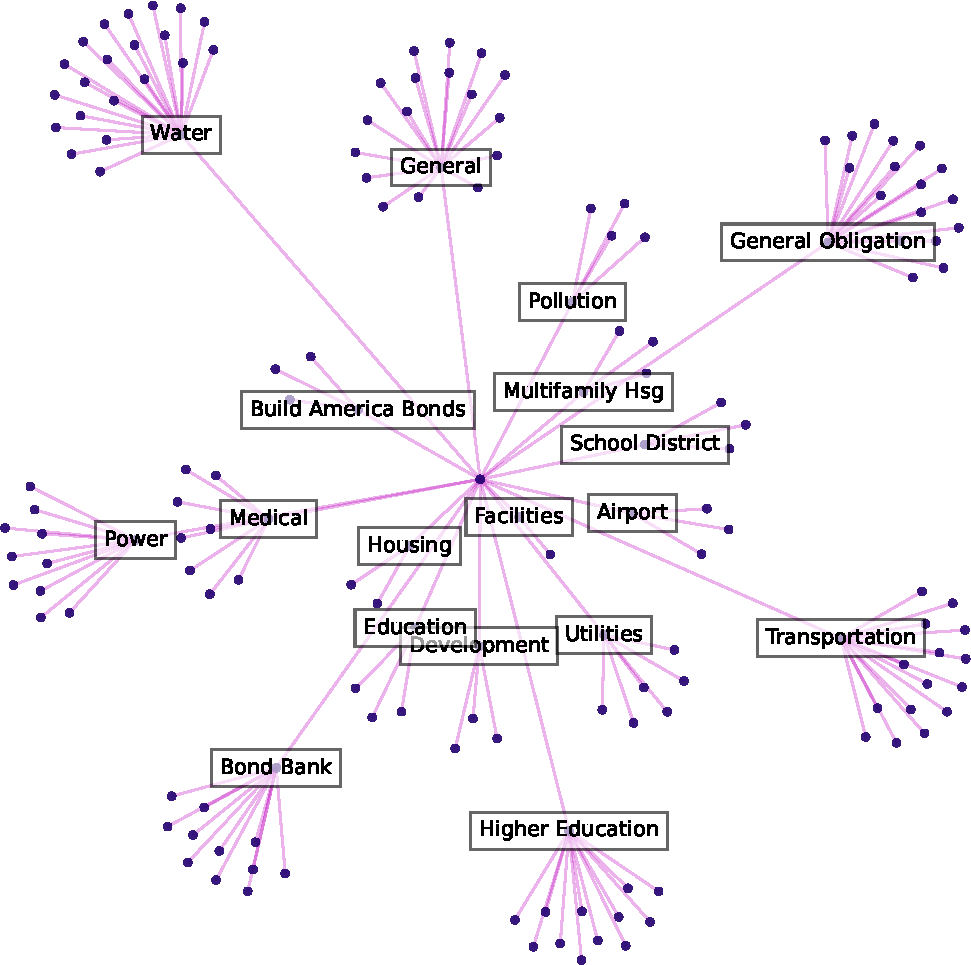
\includegraphics[width=0.8\linewidth]{Figures/bond_graph.pdf}
    \end{center}
   \caption[Graph categorising green bonds based on sector]{A representation of the graph used for categorising municipal green bonds based on the sector of the project. } 
    \label{fig:green_bond_graph}
    \vspace{1.5cm}
\end{figure} 

\begin{table}[t]
    \centering
    \def\arraystretch{1.5}
    \begin{tabular}{l p{9cm}}
        \toprule
        \textbf{Tax Status} & \textbf{Description} \\ 
        \midrule
        Fed \& St Tax-Exempt & Exempt from tax at both the federal and state level.  \\ 
        Fed Taxable/St Tax-Exempt & Taxable at the federal level, exempt at the state level.  \\ 
        Fed Tax-Exempt/St Taxable & Exempt at the federal level, taxable at the state level. \\ 
        Fed BQ/St Tax-Exempt & ``Bank Qualified'' (special provisions for large banks) at the federal level, exempt at the state level.  \\ 
        Fed Tax-Exempt & Exempt at the federal level, no information about the state level. \\ 
        AMT/St Tax-Exempt & ``Alternate Minimum Tax'' (special provision removing certain tax deductions) at the federal level, exempt at the state level. \\ 
        Fed Taxable/St Taxable & Taxable at both the federal and state level. \\ 
        \bottomrule
       \end{tabular}
        \caption[Information on the tax status of green bonds]{Further information on the possible tax status of the green bonds used in this case study.}
        \label{table:student}
\end{table}

\begin{figure}[b]  
    \begin{center}
        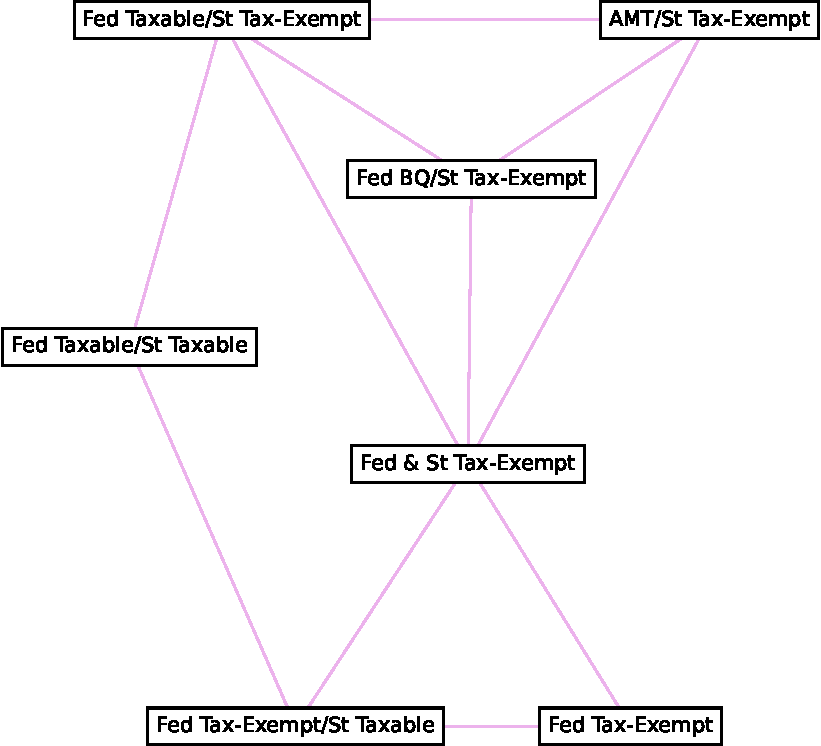
\includegraphics[width=0.66\linewidth]{Figures/tax_graph.pdf}
    \end{center}
   \caption[Graph categorising green bonds based on tax status]{A representation of the graph used for categorising municipal green bonds based on the associated tax status. Two different statuses are linked via an edge if they share at least one property in common. } 
    \label{fig:tax_graph}
\end{figure} 


\newpage 

\phantom{blabla}

\newpage


Given these factors, each bond could be associated with a particular four-dimensional coordinate: use of funds, credit rating, maturity, and tax status. With the inclusion of a time coordinate, encompassing weekly data from June 2018 to March 2023, the resulting input tensor $\Yt$ had five distinct axes, with an overall shape of $(429, 161, 8, 8, 7)$. For the KGR model, this can be interpreted as $T=429$ repeated measurements of a 4-dimensional multiway graph signal, and for the GSR model, it can be regarded as a single measurement of a 5-dimensional graph signal, with time also represented by a chain graph. \Cref{fig:bond_tensor} provides a visual representation of the tensor signal, $\Yt$, utilised in this application.

\begin{figure}[t] 
    \begin{center}
        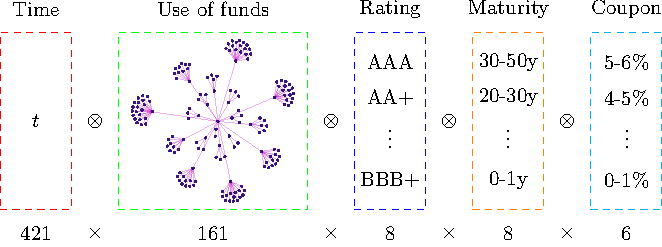
\includegraphics[width=0.9\linewidth]{Figures/bond_tensor.pdf}
    \end{center}
   \caption[A visualisation of the tensor coordinates used in the greed bond application]{A visualisation of the tensor coordinates used in this application. Rating, maturity and coupon are all represented by a chain graph, while category is represented by a tree graph as described above.} 
    \label{fig:bond_tensor}
\end{figure} 

For many specific tensor coordinates, no bond yield existed, and as such the tensor $\Yt$ was very sparse. This could be because the bond was not trading at this particular time, or because no bond ever existed with these particular characteristics. Moreover, since the parent nodes in the graph representing the use of funds are in a sense ``artificial" - serving solely to create the tree structure - no realised yield could exist there. Under the framework developed in this thesis, this does not present a problem, since we can simply allocate these coordinates as containing missing data, as specified by the binary sensing tensor $\St$. 

Additionally, certain bonds shared identical characteristics, i.e., the same use of funds, rating, maturity, and tax status. In these instances, we simply selected the bond with the longest available history and randomly broke ties. In total, we used 829 bonds (out of a theoretically possible $161 \times 8 \times 8 \times 7 = 72,128$). As many bonds did not span the total 429 weeks, this left a total missingness of $m=99.27\%$.

As previously noted, one model we employ in this case study to predict the yields is Kernel Graph Regression. This necessitates, in addition to the input tensor $\Yt$ and the sensing tensor $\St$, a matrix of explanatory variables $\X$ with shape $(T, M)$. Here, we use the treasury yields over 11 different maturities, along with core inflation, the Federal Reserve fund rate, and a simple linear variable $t$ ranging from -1 to 1, totalling $M=14$ explanatory variables. This data was obtained from the FRED API \citep{FRED2023}.


\begin{table*}[t] 
    \centering
    \def\arraystretch{1.5} 
    \begin{tabular}{@{}ccccccccc}
    \toprule
    & \multicolumn{2}{c}{Training} & \phantom{abc} & \multicolumn{2}{c}{Validation} & \phantom{abc} & \multicolumn{2}{c}{Test} \\
    \cmidrule{2-3} \cmidrule{5-6} \cmidrule{8-9}
    & MSE  & $R^2$  &&  MSE  & $R^2$ &&  MSE  & $R^2$  \\ \midrule \rule{0pt}{1cm}

    GSR & \colorbox{best!35}{0.263} & \colorbox{best!35}{0.846} && \colorbox{best!35}{0.332} & 0.819 && 0.319 & 0.823 \\ \rule{0pt}{6ex}
    
    KGR & 0.266 & 0.845 &&  0.333 & \colorbox{best!35}{0.820} && \colorbox{best!35}{0.317} & \colorbox{best!35}{0.824} \\\rule{0pt}{6ex}
    
    Ridge & 0.387 & 0.775 && 0.501 & 0.729 && 0.497 & 0.725 \\ \rule{0pt}{6ex}
    
    Lasso &  0.424 & 0.753 && 0.482 & 0.739 && 0.506 & 0.720 \\[0.5cm] 

    \bottomrule 
    \end{tabular}
    \caption[Results for bond yield experiments]{The Mean Square Error (MSE) and $R^2$ statistic from the bond yield experiment are shown for both GSR and KGR. Results are reported on the training set, the validation set, and the test set. }
    \label{tab:bond_yield_results} 
\end{table*}

Our experiment proceeded as follows. Firstly, we randomly divided the 829 bonds into a training, validation, and test set in an 80:10:10 ratio. We then trained the GSR and KGR models on the training set, using the validation set to select the optimal hyperparameters, identified using an optimisation algorithm based on the Nelder-Mead method \citep{Gao2012}. In addition, we evaluated two standard linear regression techniques, namely Ridge and Lasso \citep{Murphy2012}. In these scenarios, the yield at each moment in time for each bond was modelled as a linear combination of a constant term, the features comprising the matrix $\X$, and a one-hot encoding of each of the bond descriptors (use of funds, rating, etc). This resulted in $1 + 14 + 159 + 8 + 8 + 7 = 197$ explanatory variables for each yield. The regularisation parameter for the Ridge and Lasso models was also selected on the validation set using a straightforward line search.

The results from the experiment can be found in \cref{tab:bond_yield_results}. As can be observed, the GSR and KGR methods attain similar performance to each other, consistently outperforming the Ridge and Lasso techniques. Both also display a Mean Square Error (MSE) and $R^2$ statistic that remains relatively constant across the training, validation, and test sets, suggesting that overfitting has largely been avoided. \Cref{fig:yield_predictions_GSR,fig:yield_predictions_KGR} showcases the output of the GSR and KGR models respectively compared with the ground truth, for nine randomly representative bonds from the test set. The shaded regions represent two standard deviations of uncertainty, which is calculated by taking 20 samples from the posterior. (The method for producing these samples is explained in \cref{chap:variance}). We can observe that both GSR and KGR make broadly similar predictions, which often correlate closely with the ground truth. However, there are instances where the predictions do systematically under or overestimate the yield, for example in the upper middle, middle right, and lower middle plots. This may indicate there was hidden information about this bond not accounted for in our explanatory variables. Further investigation into the reasons for these deviations would be valuable.

\begin{figure}[t]  
    \begin{center}
        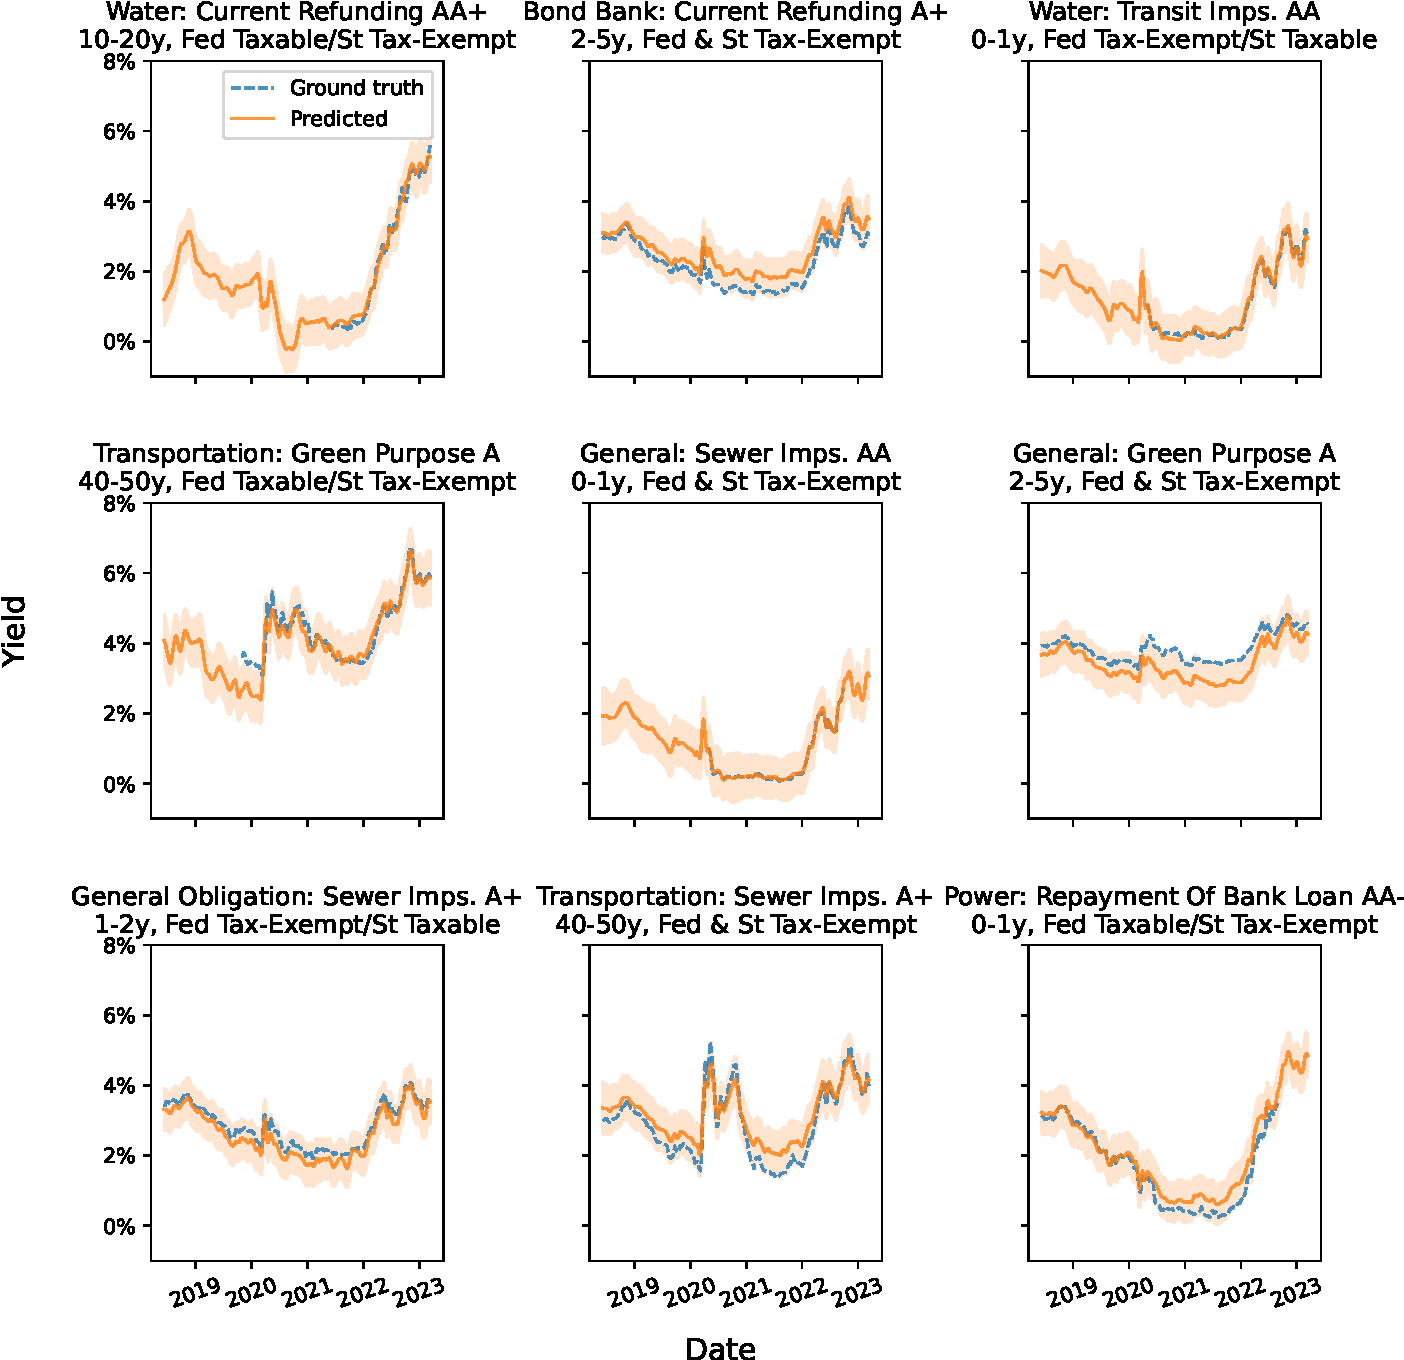
\includegraphics[width=\linewidth]{Figures/yield_predictions_GSR.pdf}
    \end{center}
   \caption[The output of the GSR model on several green bonds from the test set]{The predicted yield is shown from the GSR model, as compared to the ground truth, on a set of green bonds taken from the test set. } 
    \label{fig:yield_predictions_GSR}
\end{figure} 


\begin{figure}[t]  
    \begin{center}
        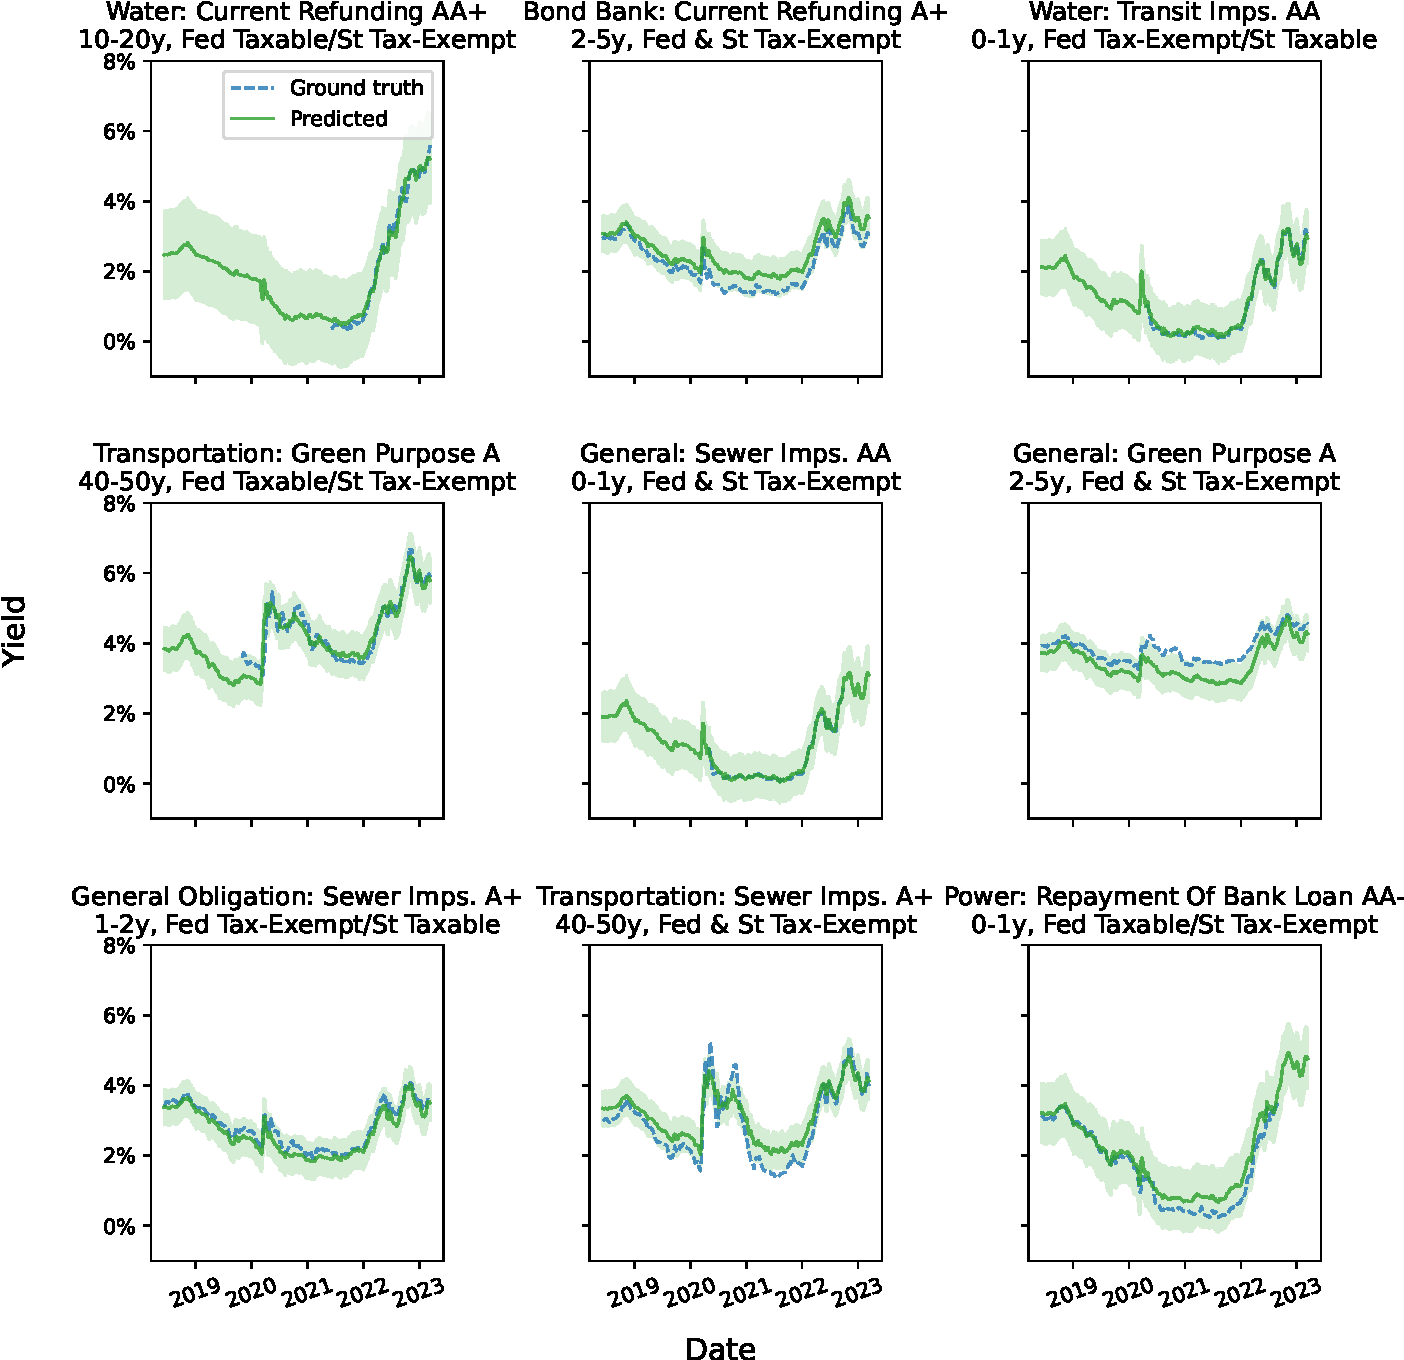
\includegraphics[width=\linewidth]{Figures/yield_predictions_KGR.pdf}
    \end{center}
   \caption[The output of the KGR model on several green bonds from the test set]{The predicted yield is shown from the KGR model as compared to the ground truth on a set of green bonds taken from the test set. } 
    \label{fig:yield_predictions_KGR}
\end{figure} 

\newpage

\section{Conclusions}

In this chapter, we have been concerned with regression and reconstruction tasks with tensor-valued signals that exist on the nodes of a $d$-dimensional Cartesian product graph, under the so-called `Multiway GSP' (MWGSP) framework \citep{Stanley2020}. We began by reviewing the concept of Cartesian product graphs in an arbitrary number of dimensions and discussed how this naturally leads to the definition of the $d$-dimensional GFT and IGFT. We also discussed the dual vector/tensor representation of multiway graph signals and highlighted the importance of efficient computation with chained Kronecker operators, presenting the PyKronecker software library for this purpose \citep{Antonian2023}. We then made the case for a restricted definition of $d$-dimensional anisotropic graph filters $g(\lambdaa)$, which are constructed as a decreasing function of a dot product between $\betaa$ and $\lambdaa$. This ensures that the resultant spectral operator can be consistently interpreted as an analytic function of a Cartesian product graph Laplacian. 

The key theoretical contribution of this chapter was to define models for graph signal reconstruction, as well as regression with exogenous and endogenous explanatory variables, for general tensor valued graph signals on $d$-dimensional Cartesian product graphs. In \cref{sec:tensor_gsr}, we reexamined the GSR model developed in \cref{chap:gsr_2d}, generalising it to $d$ dimensions. This necessitated a fresh look at the SIM and CGM methods previously developed to make them applicable to this setting. Next, in \cref{sec:kgr_dd,sec:rnc_dd} respectively we took the Kernel Graph Regression and Regression with Network Cohesion techniques, which were developed in \cref{chap:kgr_rnc_2d}, and generalised them for the multiway case. Finally, in \cref{sec:green_bonds}, we showed how the multiway KGR and GSR methods could be applied to the problem of predicting the yield of novel green bonds in a time series application. In particular, we showed that both GSR and KGR could achieve good performance, significantly outperforming the standard techniques of Ridge and Lasso regression. 

